\documentclass[11pt]{article}
\usepackage[margin=2cm]{geometry}
\usepackage{hyperref}
\usepackage{import}
\usepackage{amsmath}
\usepackage{color}
\usepackage[usenames,dvipsnames,svgnames,table]{xcolor}
\usepackage{graphicx}
\usepackage{bm}
\usepackage{float}
\usepackage[width=.75\textwidth]{caption}
\usepackage{listings}
\usepackage{tabularx, ifthen}  
\usepackage{cleveref}
\usepackage{comment}
\usepackage[backend=biber,style=numeric,citestyle=numeric]{biblatex}

\crefformat{equation}{Equation~(#2#1#3)}
\crefname{figure}{Figure}{Figures}
\crefname{table}{Table}{Tables}
\crefname{section}{Section}{}
\crefname{listing}{Listing}{}


\definecolor{gray}{rgb}{0.5, 0.5, 0.5}
\definecolor{Navy}{rgb}{0.0, 0.0, 0.5}
\definecolor{lightgray}{gray}{0.9}
\newcolumntype{R}{>{\raggedleft\arraybackslash}X}%

\definecolor{codegreen}{rgb}{0,0.6,0}
\definecolor{codegray}{rgb}{0.5,0.5,0.5}
\definecolor{codepurple}{rgb}{0.58,0,0.82}
\definecolor{backcolour}{rgb}{0.95,0.95,0.92}

\lstdefinelanguage{oofeminput}
{
morekeywords={ltrspaceboundary, node, planestress2d, libeam2d, IntElLine1, libeam3dboundary, ltrspace, libeam3d, bondlink3d, BoundaryCondition, qtrplstrslip, qplanestress2dslip, PrescribedDispSlipBCNeumannRC, PrescribedDispSlipBCDirichletRC, TransverseReinforcementConstraint, Set, StructSlipFE2Material, PrescribedDispSlipMultiple, UserDefDirichletBC}, 
morecomment=[l]{\#},
emph={coords, bc, ic, nodes, mat, crossSect, location, xy, dofidmask, doftype, mastermask, refnode, length, length_end, diameter, dirvector, dispGrad, loadTimeFunction, dofs, values, slip, slipGrad, set, conboundset, ccoord, concretevolset, rebarsets, reinfxbound, reinfybound, steelElSet,conElBoundSet, elementranges, elementboundaries, nip, filename, export_all_gps, output_selected_el_gps, use_ext_stiffness, use_num_tangent, d, dSdE, bcs, dBSdE, dRSdE, dSdS, dBSdS, dRSdS, dSdG, dBSdG, dRSdG}, 
}

\lstdefinestyle{oofem}{
  belowcaptionskip=1\baselineskip,
  frame=single,
  rulecolor=\color{gray},
  backgroundcolor=\color{lightgray},
  xleftmargin=\parindent,
  basicstyle=\ttfamily\footnotesize,
  keywordstyle=\color{red}\bfseries,
  commentstyle=\itshape, %%\color{green!40!black},
  emphstyle=\color{red},
  captionpos=b,
}

\lstdefinestyle{mystyle}{
    backgroundcolor=\color{backcolour},   
    commentstyle=\color{codegreen},
    keywordstyle=\color{magenta},
    numberstyle=\tiny\color{codegray},
    stringstyle=\color{codepurple},
    basicstyle=\ttfamily\footnotesize,
    breakatwhitespace=false,         
    breaklines=true,                 
    captionpos=b,                    
    keepspaces=true,                 
    numbers=left,                    
    numbersep=5pt,                  
    showspaces=false,                
    showstringspaces=false,
    showtabs=false,                  
    tabsize=2
}
%Commands from OOFEM input manual
\newcommand{\param}[1]{\texttt{#1}}
\newcommand{\optional}[1]{[#1]} 
\newcommand{\field}[2]{\param{#1}~{\tiny(#2)}} 
\newcommand{\optField}[2]{\optional{\field{#1}{#2}}}
\newcommand{\fieldFlag}[1]{\param{#1}} 
\newcommand{\optFieldFlag}[1]{\optional{\fieldFlag{#1}}}
\newcommand{\componentNum}{(\param{num}){\tiny(in)}} 
\newcommand{\entKeyword}[1]{*\textbf{#1}} 
\newcommand{\entKeywordInst}[1]{\textbf{#1}} 

\newcounter{rcc}
\newenvironment{record}[1][\textwidth]{\setcounter{rcc}{0}\rowcolors{1}{lightgray}{lightgray}\tabularx{#1}{llR} \hline}{\endtabularx}
\newcommand{\recentry}[2]{\ifthenelse{\value{rcc}>0}{$\backslash$ \\}{\setcounter{rcc}{1}}{#1}&{#2}&}


\title{Multiscale Modelling of Reinforced Concrete in OOFEM}
\author{Adam Sciegaj$^*$}
\date{
    $^*$ Department of Mechanics of Materials and Structures\\ 
    Faculty of Civil and Environmental Engineering\\ 
    Gdańsk University of Technology\\
    \today
}

\addbibresource{ref.bib}


\begin{document}

\maketitle

\abstract{This document summarises various aspects of multiscale modelling in the open-source C++ finite element code OOFEM developed in the course of my PhD project: \textit{``Mutltiscale modelling of reinforced concrete structures"} carried out at Chalmers University of Technology during 2015--2020. Different types of boundary conditions, finite elements and material models used within the multiscale framework are presented and the FE$^2$ modelling technique is illustrated with numerous examples. Furthermore, this document also serves as a documentation to the \href{https://github.com/adsci/oofemTests}{\texttt{oofemTests}} repository containing all examples.}

\tableofcontents
\clearpage
\section{Prerequisites}
The user should be familiar with the format of OOFEM input file. A good starting point is to consult the official manuals (especially the \textit{Input Data Format Specification}, \textit{Element Library Manual}, and \textit{Material Model Library Manual}) available at \url{https://oofem.org/doku.php?id=en:manual}. It is advised that the user first gets familiar with the OOFEM workflow (preprocessing, solving and postprocessing) on simple examples.

To make use of all features, the following is required:

\begin{itemize}
    \item A working OOFEM installation. The modified source code can be found in the \href{https://github.com/adsci/oofem}{GitHub repository}. All features (related to multiscale modelling of reinforced concrete) have been merged to the \href{https://github.com/oofem/oofem}{official OOFEM version}, so that one could be used as well. To pass all tests, OOFEM should be compiled with PETSc (\texttt{USE\_PETSC} flag), and Python support (\texttt{USE\_PYTHON\_EXTENSION} flag).

    \item CMake installation for compilation and running the tests.

    \item Some test cases require to use a PETSc solver instead of the default one. The development version of PETSc can be found at \href{https://gitlab.com/petsc/petsc}{GitLab}. The reader is referred to \href{https://www.mcs.anl.gov/petsc/}{official PETSc website} for more information on installation. The \texttt{release} branch should be cloned PETSc should be compiled with MUMPS solver. Use 

    \texttt{./configure --download-mumps --download-scalapack --download-parmetis --download-metis --download-ptscotch} 
    
    when configuring to have PETSc installed with MUMPS. If OOFEM is not compiled with PETSc, the following test cases will fail:
    \begin{itemize}
        \item \texttt{fe2Disp/planeStress/deepbeam04}
        \item \texttt{rveDisp/3D/plateBending}
        \item \texttt{rveDisp/3D/plateTension}
        \item \texttt{rveDisp/3D/sm1}
        \item \texttt{rveDisp/3D/sm2}
        \item \texttt{rveDisp/3D/sm3}
    \end{itemize}


    \item Python 3 installation. Necessary if the user wants to run an analysis on a single RVE with prescribed strain/slip history (i.e., this is not required for full FE$^2$ analysis). OOFEM should then be compiled with Python support, i.e., with the flag \texttt{USE\_PYTHON\_EXTENSION} set on. If OOFEM is not compiled with Python support, the following test cases will fail:
    \begin{itemize}
        \item \texttt{fe2Disp/planeStress/fakefe2disp}
        \item \texttt{fe2DispSlip/planeStress/fakefe2dispslip01}
        \item \texttt{fe2DispSlip/planeStress/fakefe2dispslip02}
    \end{itemize}

    \item ParaView (to be downloaded from \href{https://www.paraview.org/}{official website} and installed) can be used for postprocessing. The \texttt{*.vtu} and \texttt{*.pvd} files produced by the VTKXML output module can be used for visualizing results.

    \item SALOME (to be downloaded from \href{https://www.salome-platform.org/}{official website}) makes preprocessing much easier. Output from SALOME can be converted to OOFEM format using the \texttt{unv2oofem} tool. More information can be found \href{http://www.oofem.org/wiki/doku.php?id=unv2oofem:unv2oofem}{in OOFEM wiki}.
\end{itemize}

\clearpage
\section{Test cases}

A number of unit tests was developed during the project. 
Test cases aim to test not only each developed features, but also the FE$^2$ approach,
which makes use of many components simultaneously.
The unit tests are available in the GitHub repository \href{https://github.com/adsci/oofemTests}{\texttt{oofemTests}} and are divided into following categories:

\begin{itemize}
    \item \texttt{elements}: test of various 2D and 3D finite elements
    \item \texttt{fe2Disp}: tests of classical (plane stress) FE$^2$ analyses in 2D 
    \item \texttt{fe2DispSlip}: tests of enhanced (macroscopic strain and slip fields) FE$^2$ analyses in 2D (in plane stress)
    \item \texttt{materials}: tests of material models 
    \item \texttt{rveDisp}: tests on 2D and 3D reinforced concrete RVEs (plane stress, macroscopic Euler-Bernoulli beam, macroscopic Kirchhoff-Love plate)
    \item \texttt{rveDispSlip}: tests on 2D reinforced concrete RVEs (with boundary conditions prescribing both the strain, macroscopic reinforcement slip and slip gradient)
\end{itemize}

\noindent The easiest way to run all tests is to clone the repository and provide the path to the OOFEM executable (either \texttt{debug} or \texttt{release} version, although the \texttt{release} version is recommended for a speedy resolution) with CMake: 

\begin{lstlisting}[style=oofem]
git clone https://gitub.com/adsci/oofemTests oofemTests
cd oofemTests
cmake -DOOFEM_PATH=/path/to/oofem .
\end{lstlisting}


\noindent After that, the test suite can be run with ctest, e.g.,
\begin{lstlisting}[style=oofem]
ctest -j 8
\end{lstlisting}
\noindent runs the tests suites in parallel using 8 jobs.

\clearpage
\section{The RVE}

The Representative Volume Element (RVE) is the main building block of multiscale model. In this project, the RVE considered the plain concrete solid, the reinforcement bars, and the bond between them. 
Both 2D and 3D models of the RVE were created, but only 2D RVEs were used in full FE$^2$ analyses.
Below, the RVE models are briefly described.

\subsection{2D}
\subsubsection{Model summary}
In 2D, the RVE had a square shape with reinforcement bars arranged in a regular grid, see \cref{s}.
Depending on the size, either one, two or three reinforcing bars in each direction were considered \cite{PaperA,PaperB,PaperC}. Although in most cases both horizontal and vertical rebars were considered, \cite{Sciegaj2019semc} included examples with reinforcement only in one direction.

\begin{figure}[H]
    \centering
\def\svgwidth{0.6\textwidth}
\import{img}{rves.pdf_tex}
\caption{Examples of 2D reinforced concrete RVEs. From \cite{PaperA}.}
\label{s}
\end{figure}

Sample input files with the 2D RVE can be found e.g., in \texttt{rveDisp/2D} directory. In particular, the tests \texttt{rveDisp01, rveDisp02, rveDisp03, rveDisp04} contain input files for the smallest RVE from \cref{s}. In the same directory, Python scripts for creating the RVE mesh in SALOME and exporting it into OOFEM format are present (\texttt{rveDisp/2D/salomeAutoRVE})
The RVEs were modelled as follows:
\begin{itemize}
    \item plane stress rectangular elements (\texttt{planestress2d}) were used for the concrete solid, e.g., 
    \begin{lstlisting}[style=oofem, language=oofeminput]
planestress2d 1 nodes 4 3 46 58 13
    \end{lstlisting}
    \item beam elements with linear shape function (\texttt{libeam2d}) were used for the reinforcement bars. Note that the keyword \texttt{xy} was specified to make sure that bending happens in-plane, e.g.,
    \begin{lstlisting}[style=oofem, language=oofeminput]
libeam2d 101 nodes 2 124 125 crossSect 5 xy
    \end{lstlisting}
    \item interface elements (\texttt{IntElLine1}) were placed between the coincident nodes of concrete and beam elements to describe the bond action (along the interface), e.g.,
    \begin{lstlisting}[style=oofem, language=oofeminput]
IntElLine1 121 nodes 4 2 14 135 136  crossSect 7
    \end{lstlisting}
    \item slip across the inerface (transverse slip) was prevented \textit{strongly} by appropriate tyings between concrete and steel, e.g.,
    \begin{lstlisting}[style=oofem, language=oofeminput]
node 122 coords 3 0.0 0.0 0.0 dofidmask 3 1 2 6 doftype 3 1 0 0 
         mastermask 3 1 0 0
    \end{lstlisting}
    The transverse constraint can also be applied \textit{weakly}, see \cref{sec:trc} for more information.
    \item a \texttt{SimpleCS} cross-section and \texttt{MazarsModel} material model was used for the plane-stress concrete elements

    \item a \texttt{LayeredCS} cross-section and \texttt{MisesMat} material model was used for the steel. Layered cross-section is needed if we want to use a plasticity model for the steel.

    \item an \texttt{InterfaceCS} cross-section and \texttt{bondceb} material was used to model the interface.
\end{itemize}


\subsubsection{Analysis}
The RVE model can either be used in the FE$^2$ setting, or off-line, for analyses on the subscale level. The application of the model to full FE$^2$ analysis requires the use of special boundary conditions, which allow for efficient homogenization of the subscale results, i.e., computing the homogenized work-conjugates (stress, transfer stress, reinforcement stress). For more information on this, the reader is referred to Sections~\cref{sec:homogenization,sec:bc}. Those boundary conditions allow for efficient homogenization of the results, such as computing the homogenized stress tensor etc. 

Off-line subscale analyses should follow the usual OOFEM convention, i.e., specifying analysis type and boundary conditions. Afterwards, the results can be visualized using the \texttt{vtkxml} export module.

\subsubsection{Pertinent test cases}

Following test cases can be studied for more insight: 

\begin{itemize}
    \item \texttt{materials/bondceb01} - simple pull-out test in 2D
    \item \texttt{materials/bondceb02} - simple pull-out test in 3D
\end{itemize}

\subsection{3D}
\label{sec:3d}

Modelling of the reinforced concrete RVE in 3D involves using 3D solid tetrahedra and beam elements. Between those, 3D node-to-node interface elements are placed. 
However, before the final model is described, some requirements of the mesh are presented.

\subsubsection{Periodicity of the finite element mesh}
A modelling paradigm has been chosen so that strongly periodic boundary conditions are implicitly used. 
This, in turn requires that the mesh is also periodic.
To fulfil the periodicity requirements, all nodes present on the image boundary must have a counterpart on the mirror boundary, see \cref{fig:ltrspaceboundary}, where an example of periodicity (in $x$-direction) is shown for a solid tetrahedron element present on an image boundary.

\begin{figure}
    \centering
    \def\svgwidth{0.6\textwidth}
    \import{img}{ltrspaceboundary.pdf_tex}
    \caption{Image and mirror boundaries in the 3D RVE.}
    \label{fig:ltrspaceboundary}
\end{figure}

Note that in general, the periodicity can extend in $x$-, $y$- and $z$-directions (depending on the type of the homogenization/mode of the macroscale - see \cref{sec:homogenization})
To ensure consistency between different modes, the following convention has been used to find the mirror boundary for a cube/cuboid RVE:
\begin{itemize}
    \item We define right-handed Cartesian coordinate system with the $x$-axis to the right. The system is aligned with the cube/cuboid.
    \item All faces with outward-pointing normal unit vectors that are in \textit{opposite} direction to the axes of coordinate system are considered \textit{mirror faces}.
    \item If an edge is adjacent to \textit{two mirror faces}, it is considered an \textit{mirror edge}.
    \item The corner which belongs to \textit{mirror edges} is considered to be the \textit{mirror corner}.
    \item Mirror boundary is considered to be the \textit{union} of the mirror faces, mirror edges and mirror corner.
\end{itemize}

The periodic mapping $\varphi(\bm{x})$ maps any point outside the image boundary to a corresponding point on the image boundary. In case of points lying on the image faces, mapping is straightforward, i.e., a point on the opposite face is considered. In case of points on image edges, the point is mapped on the corresponding mirror edge with the same direction as the image edge. 
Furthermore, all image corners are mapped to the mirror corner. 
An example of edge mapping is shown in \cref{fig:periodicity}, where the mirror boundary has been marked with light yellow (faces), red (edges) and blue (corner). To make the image more legible, the mapping has been split into three direction ($x$, $y$, and $z$, going from the left)

\begin{figure}
    \centering
    \def\svgwidth{0.8\textwidth}
    \import{img}{periodicMapping.pdf_tex}
    \caption{Periodic mapping of points lying on the edges of image boundary.}
    \label{fig:periodicity}
\end{figure}


In order to use the mapping in OOFEM input files, it is necessary to be able to find a mirror node for any image node. To make that easier, a set of \textbf{switches} has been introduced. 
Switches are indicator variables which tell the program how to calculate the coordinates of the mirror node given an image node. This is done by specifying the offset between the image and mirror boundaries. 
Each switch consists of a triple of ternary values $(x,y,z)$.
Each value of the triple describes where the pertinent coordinate of the mirror node can be found:
\begin{itemize}
    \item $x=1$ means the $x$-coordinate of the image is to the right of the mirror. Accordingly, $x=-1$ means the $x$-coordinate of the image is to the left of the mirror. $x=0$ means that the $x$-coordinates of the image and the mirror are the same. 
    \item $y=1$ means the $y$-coordinate of the image is behind the mirror. Accordingly, $y=-1$ means the $y$-coordinate of the image is before the mirror. $y=0$ means that the $y$-coordinates of the image and the mirror are the same. 
    \item $z=1$ means the $z$-coordinate of the image is above the mirror. Accordingly, $z=-1$ means the $z$-coordinate of the image is below the mirror. $z=0$ means that the $z$-coordinates of the image and the mirror are the same.
\end{itemize}

For example, if we consider the image face shown in \cref{fig:ltrspaceboundary}, we see that all points on it are situated to the right to the mirror boundary. At the same time, the $y$- and $z$-coordinates of the mirror nodes are the same as those of the image nodes. This corresponds to the indicator triple $(x = 1, y=0, z = 0)$.

As each value in the triple is either $-1$, $0$, or $1$, there exist in total 27 different switches. 
However, as the triple $(0,0,0)$ is an identity mapping, we don't consider that case. The remaining $26$ switches are are summarised in \cref{tab:switches}. To summarize, all switches used in mapping for points located on the image boundary are shown in \cref{fig:switches}. For clarity, periodicity in each direction is shown separately.

\begin{table}[]
    \caption{Switches used in periodic mapping.}
    \centering
    \begin{tabular}{|c|l|l|l|}
    \hline
    \textbf{Switch} & $x$ & $y$ & $z$ \\ \hline
    \textbf{1}          & -1  & -1  & -1  \\ \hline
    \textbf{2}          & -1  & -1  & 0   \\ \hline
    \textbf{3}          & -1  & -1  & 1   \\ \hline
    \textbf{4}          & -1  & 0   & -1  \\ \hline
    \textbf{5}          & -1  & 0   & 0   \\ \hline
    \textbf{6}          & -1  & 0   & 1   \\ \hline
    \textbf{7}          & -1  & 1   & -1  \\ \hline
    \textbf{8}          & -1  & 1   & 0   \\ \hline
    \textbf{9}          & -1  & 1   & 1   \\ \hline
    \textbf{10}         & 0   & -1  & -1  \\ \hline
    \textbf{11}         & 0   & -1  & 0   \\ \hline
    \textbf{12}         & 0   & -1  & 1   \\ \hline
    \textbf{13}         & 0   & 0   & -1  \\ \hline
    \textbf{14}         & 0   & 0   & 1   \\ \hline
    \textbf{15}         & 0   & 1   & -1  \\ \hline
    \textbf{16}         & 0   & 1   & 0   \\ \hline
    \textbf{17}         & 0   & 1   & 1   \\ \hline
    \textbf{18}         & 1   & -1  & -1  \\ \hline
    \textbf{19}         & 1   & -1  & 0   \\ \hline
    \textbf{20}         & 1   & -1  & 1   \\ \hline
    \textbf{21}         & 1   & 0   & -1  \\ \hline
    \textbf{22}         & 1   & 0   & 0   \\ \hline
    \textbf{23}         & 1   & 0   & 1   \\ \hline
    \textbf{24}         & 1   & 1   & -1  \\ \hline
    \textbf{25}         & 1   & 1   & 0   \\ \hline
    \textbf{26}         & 1   & 1   & 1   \\ \hline
    \end{tabular}
    \label{tab:switches}
\end{table}

\begin{figure}
    \centering
    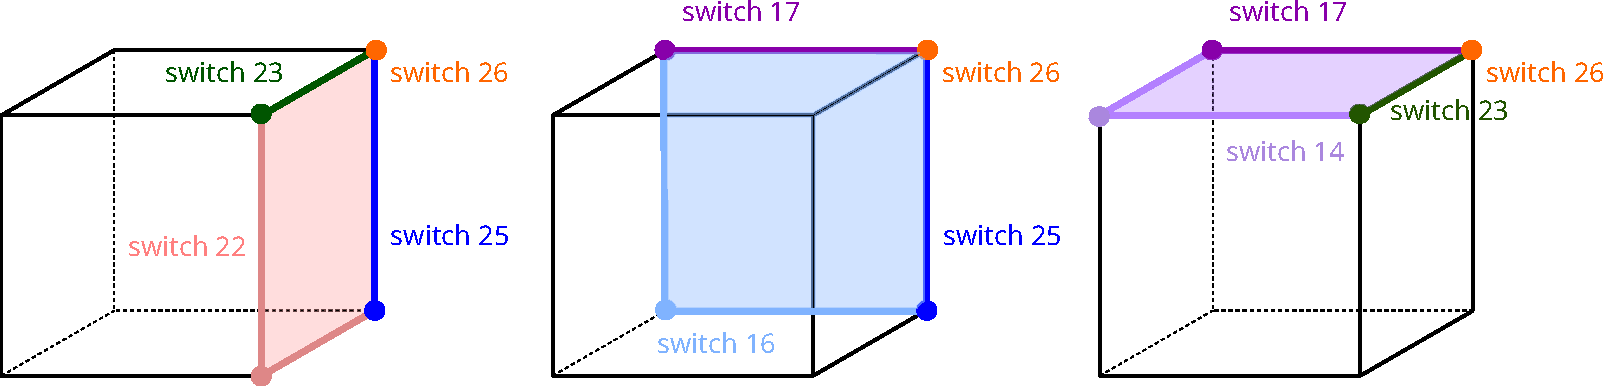
\includegraphics[width=0.85\textwidth]{img/switches.pdf}
    \caption{Switches used in periodic mapping (separately for $x$-, $y$- and $z$-direction, from left to right).}
    \label{fig:switches}
\end{figure}

\subsubsection{RVE master node}

Each RVE needs to have a master node. 
This special node acts as a link between the macroscale and the subscale. Boundary conditions can be set on the master node, i.e., prescribing certain components of macroscopic tensors. 
After solving the RVE problem, reactions in the master node correspond to the homogenized work-conjugates, e.g., stresses, normal forces and bending moments. The master node needs to fulfil following requirements requirements:
\begin{itemize}
    \item the coordinates of the master node should be $(L_x, L_y, L_z)$, i.e., length, width and height of the RVE, where $L_i$ is the side length of the RVE in direction $i$. These values are used together with the switches to calculate the positions of the mirror nodes,
    \item no finite element should be explicitly connected to this node.
    \item the exception to the above are boundary elements (\texttt{ltrspaceboundary, libeam3dboundary} and derived classes), which have the master node as their fifth node
    (more on boundary elements in the following subsection),
    \item it has a \texttt{dofidmask} according to \cref{tab:modes}. More information on macroscale modes can be found in \cref{sec:homogenization}. An example definition is provided in \cref{lst:masternode}, where a master node with number 126 has been defined. 
    The node has coordinates (0.1, 0.1, 0.1), meaning that the RVE is a cube with a side length of $0.1$. \texttt{dofidmask} of this node specifies a full 3D mode, and boundary condition 2 is prescribed on each degree of freedom.
\end{itemize}

\begin{lstlisting}[style=oofem,language=oofeminput, caption={Example of master node definition}, label=lst:masternode]
node 126 coords 3 1.000000e-01 1.000000e-01 1.000000e-01 
         dofidmask 9 31 38 36 39 32 34 37 35 33 bc 9 2 2 2 2 2 2 2 2 2
\end{lstlisting}

\begin{table}
    \centering
    \caption{Macroscopic modes and corresponding \texttt{dofidmask}s.}
    \begin{tabular}{|l|l|l|l|}
    \hline
    \textbf{Mode}     & \textbf{Macroscopic components}                                                                                                                                                                                                                                                                      & \textbf{ndofs} & \multicolumn{1}{c|}{\texttt{dofidmask}}                    \\ \hline
    Truss    & $\bar{\varepsilon}_{xx}$                                                                                                                                                                                                                                                                             & \texttt{1}              & \texttt{31}                            \\ \hline
    Membrane & \begin{tabular}[c]{@{}l@{}}$\bar{\varepsilon}_{xx}$, $\bar{\varepsilon}_{xy}$, $\bar{\varepsilon}_{yx}$, $\bar{\varepsilon}_{yy}$\end{tabular}                                                                                                                                                      & \texttt{4}              & \texttt{31 38 39 32}                   \\ \hline
    3DVoigt  & \begin{tabular}[c]{@{}l@{}}$\bar{\varepsilon}_{xx}$, $\bar{\varepsilon}_{yy}$, $\bar{\varepsilon}_{zz}$, $\bar{\gamma}_{yz}$, $\bar{\gamma}_{xz}$, $\bar{\gamma}_{xy}$\end{tabular}                                                                                                                  & \texttt{6}              & \texttt{31 32 33 40 41 42}             \\ \hline
    3D       & \begin{tabular}[c]{@{}l@{}}$\bar{\varepsilon}_{xx}$, $\bar{\varepsilon}_{xy}$, $\bar{\varepsilon}_{xz}$, \\ $\bar{\varepsilon}_{yx}$,  $\bar{\varepsilon}_{yy}$, $\bar{\varepsilon}_{yz}$, \\ $\bar{\varepsilon}_{zx}$,  $\bar{\varepsilon}_{zy}$, $\bar{\varepsilon}_{zz}$\end{tabular}                 & \texttt{9}              & \texttt{31 38 36 39 32 34 37 35 33}    \\ \hline
    Beam     & \begin{tabular}[c]{@{}l@{}}$\bar{\varepsilon}_{xx}$, $\bar{\varepsilon}_{zx}$,$\bar{\kappa}_{xx}$\end{tabular}                                                                                                                                                                                    & \texttt{3}              & \texttt{31 37 43}                      \\ \hline
    Plate    & \begin{tabular}[c]{@{}l@{}}$\bar{\varepsilon}_{xx}$, $\bar{\varepsilon}_{xy}$, $\bar{\varepsilon}_{yx}$, $\bar{\varepsilon}_{yy}$, \\ $\bar{\varepsilon}_{zx}$, $\bar{\varepsilon}_{zy}$, \\ $\bar{\kappa}_{xx}$,  $\bar{\kappa}_{yy}$, $\bar{\kappa}_{xy}$, $\bar{\kappa}_{yx}$\end{tabular} & \texttt{10}             & \texttt{31 38 39 32 37 35 43 44 49 50} \\ \hline
    \end{tabular}
    \label{tab:modes}
\end{table}




\subsubsection{Boundary elements}

All element with at least one node located on the image boundary need to be boundary elements.
Boundary elements are a special class of element, which will use the mirror nodes when assembling stiffness matrices and internal force vectors. 
At the moment, there are 2 classes that implement boundary elements: 
\begin{itemize}
    \item \texttt{ltrspaceboundary} and derived classes implement a boundary version of the \texttt{ltrspace} 4-node tetrahedral solid element,
    \item \texttt{libeam3dboundary} and derived classes implement a boundary version of the \texttt{libeam3d} 2-node beam element.
\end{itemize}

Boundary elements have the same number of nodes as the parent, plus the RVE master node.
Also, a special \texttt{location} keyword needs to be used when defining boundary elements. Following the keyword, an integer array with switches corresponding to each node is placed. For example, \cref{lst:ltrspaceboundary}
defines a couple of boundary elements. The \texttt{ltrspaceboundary} element with number 14 uses 4 normal nodes (99, 9, 45, 90) and the master node (126). \texttt{location} keyword specifies that node 9 has switch 17, node 45 has switch 14, and node 90 has switch 22. The first node (99) does not have a switch, which means it is not located on the image boundary. 
Similarly, the \texttt{libeam3dboundary} element with number 8 has 2 normal nodel (8, 5) and the master node (126). Note that the master node in an RVE is common for all boundary elements. Reference node 10 is used to orient the beam correctly in space (the reader is referred to \textit{OOFEM Element Library Manual}).

\begin{lstlisting}[style=oofem, language=oofeminput, caption={Example of boundary elements definition}, label=lst:ltrspaceboundary]
# ltrspaceboundary element definition
ltrspaceboundary 14 nodes 5 99 9 45 90 126 location 4 0 17 14 22
# libeam3dboundary element definition
libeam3dboundary 8 nodes 3 8 5 126 refnode 10 crossSect 1 location 2 0 22
\end{lstlisting}



Knowing the switches and the sizes of the RVE (indirectly through the coordinates of the master node), the element can compute coordinates of all mirror nodes. Those are later used to construct the stiffness matrix and internal force vectors, as described in more detail in \cite{PaperE}.
For each parent element, six different types of boundary elements were implemented, depending on the macroscopic mode:

\begin{table}[]
    \centering
    \caption{Boundary element names and pertinent test cases.}
    \begin{tabular}{|l|l|l|}
    \hline
    \textbf{Mode} & \textbf{Element name}                                                                                                  & \textbf{Test case}                                                                                                            \\ \hline
    Truss         & \begin{tabular}[c]{@{}l@{}}\texttt{ltrspaceboundarytruss}, \\ \texttt{libeam3dboundarytruss}\end{tabular}       & \begin{tabular}[c]{@{}l@{}}\texttt{elements/ltrspaceboundary01}, \\ \texttt{elements/libeam3dboundary01}\end{tabular} \\ \hline
    Membrane      & \begin{tabular}[c]{@{}l@{}}\texttt{ltrspaceboundarymembrane},\\ \texttt{libeam3dboundarymembrane}\end{tabular} & \begin{tabular}[c]{@{}l@{}}\texttt{elements/ltrspaceboundary02}, \\ \texttt{elements/libeam3dboundary02}\end{tabular} \\ \hline
    3DVoigt       & \begin{tabular}[c]{@{}l@{}}\texttt{ltrspaceboundaryvoigt},\\ \texttt{libeam3dboundaryvoigt}\end{tabular}       & \begin{tabular}[c]{@{}l@{}}\texttt{elements/ltrspaceboundary03}, \\ \texttt{elements/libeam3dboundary03}\end{tabular} \\ \hline
    3D            & \begin{tabular}[c]{@{}l@{}}\texttt{ltrspaceboundary},\\ \texttt{libeam3dboundary}\end{tabular}                 & \begin{tabular}[c]{@{}l@{}}\texttt{elements/ltrspaceboundary04}, \\ \texttt{elements/libeam3dboundary04}\end{tabular} \\ \hline
    Beam          & \begin{tabular}[c]{@{}l@{}}\texttt{ltrspaceboundarybeam},\\ \texttt{libeam3dboundarybeam}\end{tabular}         & \begin{tabular}[c]{@{}l@{}}\texttt{elements/ltrspaceboundary05}, \\ \texttt{elements/libeam3dboundary05}\end{tabular} \\ \hline
    Plate         & \begin{tabular}[c]{@{}l@{}}\texttt{ltrspaceboundaryplate},\\ \texttt{libeam3dboundaryplate}\end{tabular}    & \begin{tabular}[c]{@{}l@{}}\texttt{elements/ltrspaceboundary06}, \\ \texttt{elements/libeam3dboundary06}\end{tabular} \\ \hline
    \end{tabular}
    \end{table}


\subsubsection{Model summary}

A sample input file with the 3D RVE can be found e.g., in \texttt{rveDisp/3D} directory. In particular, the tests \texttt{beamTension, beamBending, plateTension, plateBending} contain input files for a complete reinforced concrete RVE. As a reminder, it is required that the RVE has a periodic mesh. More details on mesh generation can be found in \cite{PaperE}.
The RVEs were modelled as follows:
\begin{itemize}
    \item solid tetrahedral elements (\texttt{ltrspace}) were used for the concrete solid \textbf{not on the image boundary}, e.g., 
    \begin{lstlisting}[style=oofem, language=oofeminput]
ltrspace 1481 nodes 4 1605 6933 1389 3801 
    \end{lstlisting}
    \item 3D beam elements with linear shape function (\texttt{libeam3d}) were used for the reinforcement bars \text{not on the image boundary}, e.g.,
    \begin{lstlisting}[style=oofem, language=oofeminput]
libeam3d 44477 nodes 2 7041 7042 refnode 7069
    \end{lstlisting}
    \item 3D node-to-node interface elements (\texttt{bondlink3d}) were placed between the nearest nodes of concrete and beam elements to describe the bond action (along the interface), e.g.,
    \begin{lstlisting}[style=oofem, language=oofeminput]
bondlink3d 44506 nodes 2 7043 4719 dirvector 3 1.00e+00 0.00e+00 0.00e+00 
                 length 9.946627e-03 length_end 4.913651e-02 diameter 1.60e-02    \end{lstlisting}
    (\param{dirvector} defines a unit vector along the direction of the reinforcement bar with diameter specified by \param{diameter}. Parameter \param{length} defines the length of the interface pertinent to this element - it is a portion of the overall length of the rebar in the RVE)
    \item a \texttt{SimpleCS} cross-section and \texttt{idm1} material model was used for the solid concrete elements

    \item a \texttt{FiberedCS} cross-section and \texttt{MisesMat} material model was used for the steel. Fibered cross-section is needed if we want to use a plasticity model for the steel in 3D.

    \item an \texttt{InterfaceCS} cross-section and \texttt{linkslip} material was used to model the interface.
\end{itemize}

\subsubsection{Analysis}
The RVE model can only be used for analyses on the subscale level. Macroscopic quantities (such as stress tensor components, slopes or curvatures) can be prescribed on the RVE by applying a suitable boundary condition on the degree of freedom of the master node listed in \cref{tab:modes}. 
The effective (homogenized) quantities can then be obtained as reactions in the master node.


\subsubsection{Pertinent test cases}

Following test cases can be studied for more insight: 
\begin{itemize}
    \item \texttt{elements/bond\_link\_1} - test of \param{bondlink3d} element
    \item \texttt{elements/bond\_link\_2} - test of \param{bondlink3d} element
    \item \texttt{elements/bond\_link\_3} - test of \param{bondlink3d} element
    \item \texttt{elements/ltrspaceboundary01} - test of \param{ltrspaceboundarytruss} element
    \item \texttt{elements/ltrspaceboundary02} - test of \param{ltrspaceboundarymembrane} element
    \item \texttt{elements/ltrspaceboundary03} - test of \param{ltrspaceboundaryvoigt} element
    \item \texttt{elements/ltrspaceboundary04} - test of \param{ltrspaceboundary} element
    \item \texttt{elements/ltrspaceboundary05} - test of \param{ltrspaceboundarybeam} element
    \item \texttt{elements/ltrspaceboundary06} - test of \param{ltrspaceboundaryplate} element
    \item \texttt{elements/libeadm3dboundary01} - test of \param{libeam3dboundarytruss} element
    \item \texttt{elements/libeadm3dboundary02} - test of \param{libeam3dboundarymembrane} element
    \item \texttt{elements/libeadm3dboundary03} - test of \param{libeam3dboundaryvoigt} element
    \item \texttt{elements/libeadm3dboundary04} - test of \param{libeam3dboundary} element
    \item \texttt{elements/libeadm3dboundary05} - test of \param{libeam3dboundarybeam} element
    \item \texttt{elements/libeadm3dboundary06} - test of \param{libeam3dboundaryplate} element
    \item \texttt{materials/linkslip01} - test of \param{linkslip} material model
\end{itemize}

\clearpage
\section{Macroscale modes}
\label{sec:homogenization}

This section follows closely the description of different multiscale models for reinforced concrete structures given in \cite{Sciegaj2020phd}, to which the reader is kindly referred. 
Instead of focusing on mathematical derivations, only summary of the information will be given here. 

The basic layout of the FE$^2$ multiscale modelling technique is presented in \cref{fig:fe2}. For a given point in the large-scale model, the effective field (e.g., strain) is imposed on the RVE via suitable boundary conditions. 
Subsequently, the RVE problem is solved, and the subscale results are \textit{homogenized} and brought back to the large-scale. 
Use of different types of boundary conditions on the RVE in OOFEM will be covered in \cref{sec:bc}, whereas this section will focus on the process of formatting the prolonged fields to be used in suitable boundary conditions. 
A few macroscale modes have already been presented in \cref{tab:modes} according with the macroscopic components that are prolonged onto the RVE. Below, a few macroscale modes used within the project are presented in more detail. 

\begin{figure}[H]
    \centering
    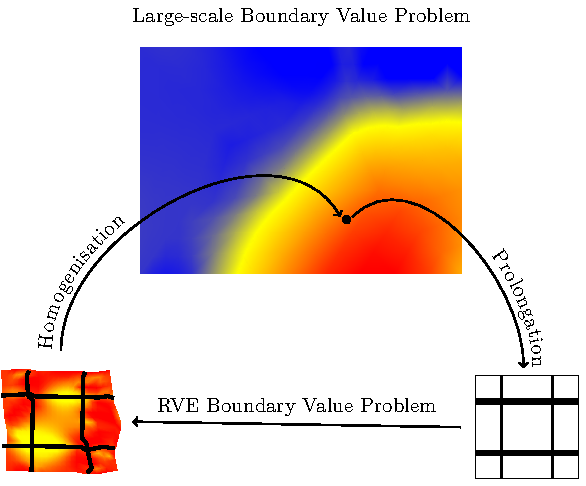
\includegraphics[width=0.6\textwidth]{img/fe2.pdf}
    \caption{FE$^2$ scheme. From \cite{Sciegaj2020phd}.}
    \label{fig:fe2}
\end{figure}

\subsection{Plane stress} 

In plane stress, the unknown large-scale field is the displacement ($\bm{\bar{u}} = [\bar{u} \quad \bar{v}]$). This field is prolonged onto the RVE via the strain tensor (or displacement gradient):
\begin{equation}
    \bm{\bar{\varepsilon}} = \left[ \bm{\bar{u}} \otimes \nabla \right] = 
    \begin{bmatrix}
        \bar{\varepsilon}_{xx} & \bar{\varepsilon}_{xy}\\
        \bar{\varepsilon}_{yx} & \bar{\varepsilon}_{yy} 
    \end{bmatrix}  =
    \begin{bmatrix}
        \dfrac{\partial \bar{u}}{\partial x} & \dfrac{\partial \bar{u}}{\partial y} \\
        \dfrac{\partial \bar{v}}{\partial x}  & \dfrac{\partial \bar{v}}{\partial y}  
       \end{bmatrix} 
\end{equation}

\noindent All we need in the 2D plane stress setting is a way to prescribe a given strain tensor on the RVE. This is done via the keyword \param{dispGrad} used in boundary conditions (\cref{sec:bc}). The keyword is followed by the strain tensor $\bm{\bar{\varepsilon}}$ entered as a real matrix according to the OOFEM Input specification. Note that the matrix is specified in row major order, i.e., the columns are separated by spaces, and the rows are separated by semicolons. For example, the following strain tensor is expressed in the OOFEM format in \cref{lst:dispGrad}:

\begin{equation*}
    \bm{\bar{\varepsilon}} = 
    \begin{bmatrix}
        0.3 \cdot  10^{-6} & 0.4 \cdot  10^{-6}\\
        0.4 \cdot  10^{-6} & -0.5 \cdot  10^{-6}
       \end{bmatrix}
\end{equation*}

\begin{lstlisting}[style=oofem,language=oofeminput, label=lst:dispGrad, caption={OOFEM input format for $\bm{\bar{\varepsilon}}$.}]
dispGrad 2 2 {0.3e-6 0.4e-6; 0.4e-6 -0.5e-6}
\end{lstlisting}


\noindent The homogenized values (stress tensor) can be computed as the average stress over the volume of the RVE, see \cite{PaperA} for details on how to do it. This can be useful when studying a single RVE. However, it is not necessary to calculate the homogenized stresses explicitly in the FE$^2$ analysis, as this is handled automatically by the boundary conditions.


\subsection{Euler-Bernoulli beam}

For the Euler-Bernoulli beam problem on the macroscale, the unknown fields are the longitudinal displacement ($\bar{u}$) and the deflection ($\bar{w}$).The prolonged quantities are the longitudinal strain ($\bar{\varepsilon}_{xx}$), the slope ($\bar{\varepsilon}_{zx}$) and the curvature ($\bar{\kappa}_{xx}$). Those components are defined as:

\begin{eqnarray}
    \bar{\varepsilon}_{xx} = \dfrac{\partial \bar{u}}{\partial x} \\
    \bar{\varepsilon}_{zx} = \dfrac{\partial \bar{w}}{\partial x} \\
    \bar{\kappa}_{xx} = \dfrac{\partial^2 \bar{w}}{\partial x^2}
\end{eqnarray}

\noindent Unlike the 2D plane stress case, no suitable multiscale boundary conditions were explicitly implemented in OOFEM. This prevents running a full FE$^2$ analysis for macroscopic beam elements at the moment. 
However, the macroscopic fields can be directly prescribed on the RVE via suitable degrees of freedom of the master node (see \cref{tab:modes}). 
This way, the macroscopic quantities are prescribed using \textbf{strongly periodic boundary conditions} (see \cref{sec:bc}), and subscale analysis on the RVE level can still be performed. 
This can be done using the conventional \texttt{BoundaryCondition} class in OOFEM. For example, prescribing the macroscopic components corresponds to the input shown in \cref{lst:macroBeam}. In the following, node 9018 is the master node of the RVE:

\begin{equation*}
    \left[ \bar{\varepsilon}_{xx} \quad \bar{\varepsilon}_{zx} \quad \bar{\kappa}_{xx} \right] = \left[ 0.3 \quad 0.0 \quad 1.0 \right]
\end{equation*}

\begin{lstlisting}[style=oofem,language=oofeminput, caption={OOFEM input format in case of an Euler-Bernoulli problem at macroscale.}, label=lst:macroBeam]
# set 1 contains the master node
BoundaryCondition 1 loadTimeFunction 1 dofs 3 31 37 43 values 3 0.3 0 1 set 1
Set 1 nodes 1 9018
\end{lstlisting}

\noindent The homogenized quantities (normal force, shear force and bending moment) can be obtained as reaction forces in the master node (on the pertinent degrees of freedom). Note that some rescaling with the RVE size might be necessary to get the actual values of the forces.

\subsubsection{Pertinent test cases}
Following test cases can be studied for more insight: 
\begin{itemize}
    \item \texttt{rveDisp/3D/macroBeam01} - prescribing macroscopic input on the 3D RVE (only solid elements)
    \item \texttt{rveDisp/3D/macroBeam02} - prescribing macroscopic input on the 3D RVE (only solid elements)
    \item \texttt{rveDisp/3D/macroBeam03} - prescribing macroscopic input on the 3D RVE (only solid elements)
    \item \texttt{rveDisp/3D/beamTension} - tension test on a 3D RVE (reinforced concrete). Presented in \cite{PaperE}.
    \item \texttt{rveDisp/3D/beamBending} - bending test on a 3D RVE (reinforced concrete). Presented in \cite{PaperE}.

\end{itemize}


\subsection{Kirchhoff-Love plate}

For the Kirchhoff-Love plate problem on the macroscale, the unknown fields are the longitudinal displacements ($\bar{u}, \bar{v}$) and the deflection ($\bar{w}$).The prolonged quantities are the membrane strains ($\bar{\varepsilon}_{xx}, \bar{\varepsilon}_{xy}, \bar{\varepsilon}_{yx}, \bar{\varepsilon}_{yy}$), the slopes ($\bar{\varepsilon}_{zx}, \bar{\varepsilon}_{zy}$) and the curvatures ($\bar{\kappa}_{xx}, \bar{\kappa}_{xy}, \bar{\kappa}_{yx}, \bar{\kappa}_{xx}$). Those components are defined as:

\begin{eqnarray}
    \begin{bmatrix}
        \bar{\varepsilon}_{xx} & \bar{\varepsilon}_{xy}\\
        \bar{\varepsilon}_{yx} & \bar{\varepsilon}_{yy} 
    \end{bmatrix}  =
    \begin{bmatrix}
        \dfrac{\partial \bar{u}}{\partial x} & \dfrac{\partial \bar{u}}{\partial y} \\
        \dfrac{\partial \bar{v}}{\partial x}  & \dfrac{\partial \bar{v}}{\partial y}  
       \end{bmatrix}  \\
    \left[ \bar{\varepsilon}_{zx} \quad \bar{\varepsilon}_{zy} \right] = \left[ \dfrac{\partial \bar{w}}{\partial x} \quad  \dfrac{\partial \bar{w}}{\partial y} \right]\\
    \begin{bmatrix}
        \bar{\kappa}_{xx} & \bar{\kappa}_{xy}\\
        \bar{\kappa}_{yx} & \bar{\kappa}_{yy} 
    \end{bmatrix}  =
    \begin{bmatrix}
        \dfrac{\partial^2 \bar{w}}{\partial x^2} & \dfrac{\partial^2 \bar{w}}{\partial x \partial y} \\
        \dfrac{\partial^2 \bar{w}}{\partial y \partial x}  & \dfrac{\partial^2 \bar{w}}{\partial y^2}  
       \end{bmatrix}
\end{eqnarray}

\noindent Unlike the 2D plane stress case, no suitable multiscale boundary conditions were explicitly implemented in OOFEM. This prevents running a full FE$^2$ analysis for macroscopic plate elements at the moment. 
However, the macroscopic fields can be directly prescribed on the RVE via suitable degrees of freedom of the master node (see \cref{tab:modes}). 
This way, the macroscopic quantities are prescribed using \textbf{strongly periodic boundary conditions} (see \cref{sec:bc}), and subscale analysis on the RVE level can still be performed. 
This can be done using the conventional \texttt{BoundaryCondition} class in OOFEM. For example, prescribing the macroscopic components corresponds to the input shown in \cref{lst:macroPlate}. In the following, node 2835 is the master node of the RVE:

\begin{equation*}
    \left[ \bar{\varepsilon}_{xx}, \bar{\varepsilon}_{xy}, \bar{\varepsilon}_{yx}, \bar{\varepsilon}_{yy}, \bar{\varepsilon}_{zx}, \bar{\varepsilon}_{zy}, \bar{\kappa}_{xx}, \bar{\kappa}_{yy}, \bar{\kappa}_{xy}, \bar{\kappa}_{yx} \right] = \left[ 0.3, 0 , 0 , -0.5 , 0 , 0 , 0.5 , -1.0 , 0 , 0 \right]
\end{equation*}

\begin{lstlisting}[style=oofem,language=oofeminput, caption={OOFEM input format in case of an Kirchhoff-Love problem at macroscale.}, label=lst:macroPlate]
# set 1 contains the master node
BoundaryCondition 1 loadTimeFunction 1 dofs 10 31 38 39 32 37 35 43 44 49 50 
                    values 10 0.3 0 0 -0.5 0 0 0.5 -1 0 0 set 1
Set 1 nodes 1 2835
\end{lstlisting}

\noindent The homogenized quantities (membrane forces, shear forces and bending moments) can be obtained as reaction forces in the master node (on the pertinent degrees of freedom). Note that some rescaling with the RVE size might be necessary to get the actual values of the forces.

\subsubsection{Pertinent test cases}
Following test cases can be studied for more insight: 
\begin{itemize}
    \item \texttt{rveDisp/3D/macroPlate01} - prescribing macroscopic input on the 3D RVE (only solid elements)
    \item \texttt{rveDisp/3D/macroPlate02} - prescribing macroscopic input on the 3D RVE (only solid elements)
    \item \texttt{rveDisp/3D/macroPlate03} - prescribing macroscopic input on the 3D RVE (only solid elements)
    \item \texttt{rveDisp/3D/plateTension} - tension test on a 3D RVE (reinforced concrete).
    \item \texttt{rveDisp/3D/plateBending} - bending test on a 3D RVE (reinforced concrete). Presented in \cite{PaperE}.
    \item \texttt{rveDisp/3D/sm1} - uniaxial bending test SM1. Presented in \cite{PaperE}.
    \item \texttt{rveDisp/3D/sm2} - uniaxial bending (with membrane loads) test SM2. Presented in \cite{PaperE}.
    \item \texttt{rveDisp/3D/sm3} - biaxial bending test SM2. Presented in \cite{PaperE}.
\end{itemize}


\subsection{Maroscopic reinforcement slip}
\label{sec:macroslip}

One enhancement that was introduced in the project at the macroscale (in plane stress) is the 
enrichment by the macroscopic reinforcement slip field, $\bm{\bar{s}} = \left[ \bar{s}_x \quad \bar{s}_y \right]$. 
The idea behind introduction of the new macroscopic field was to allow for the transfer of reinforcement slip across macroscopic elements. The macroscopic slip represents the displacement of the reinforcement grid relative to the concrete, see \cref{fig:macroslip}.

\begin{figure}[H]
    \centering
    \def\svgwidth{0.2\textwidth}
    \import{img}{macroSlip.pdf_tex}
    \caption{Physical interpretation of the macroscopic slip field. From \cite{PaperB}.}
    \label{fig:macroslip}
\end{figure}

\noindent Before (in plane stress case), only the displacement gradient was needed as input to the RVE problem. Now, due to the extra macroscopic field, two additional components are necessary. Therefore, the following are needed as the input for boundary conditions on the RVE problem:

\begin{itemize}
    \item strain tensor (displacement gradient). This component is the same as previously.
    \begin{equation}
        \bm{\bar{\varepsilon}} = \left[ \bm{\bar{u}} \otimes \nabla \right] = 
        \begin{bmatrix}
            \bar{\varepsilon}_{xx} & \bar{\varepsilon}_{xy}\\
            \bar{\varepsilon}_{yx} & \bar{\varepsilon}_{yy} 
        \end{bmatrix}  =
        \begin{bmatrix}
            \dfrac{\partial \bar{u}}{\partial x} & \dfrac{\partial \bar{u}}{\partial y} \\
            \dfrac{\partial \bar{v}}{\partial x}  & \dfrac{\partial \bar{v}}{\partial y}  
           \end{bmatrix} 
    \end{equation}    
    \item macroscopic slip field:
    \begin{equation}
        \bm{\bar{s}} = \left[ \bar{s}_x \quad \bar{s}_y \right]
    \end{equation}
    \item slip gradient (gradient of the macroscopic slip field):
    \begin{equation}
        \bm{\bar{g}} = \left[ \bm{\bar{s}} \otimes \nabla \right] = 
        \begin{bmatrix}
            \bar{g}_{xx} & \bar{g}_{xy}\\
            \bar{g}_{yx} & \bar{g}_{yy} 
        \end{bmatrix}  =
        \begin{bmatrix}
            \dfrac{\partial \bar{s}_x}{\partial x} & \dfrac{\partial \bar{s}_x}{\partial y} \\
            \dfrac{\partial \bar{s}_y}{\partial x}  & \dfrac{\partial \bar{s}_y}{\partial y}  
           \end{bmatrix} 
    \end{equation}
\end{itemize}

\noindent The corresponding work conjugates are:
\begin{itemize}
    \item $\bm{\bar{\sigma}}$ - effective stress (conjugated with strain),
    \item $\bm{\bar{\tau}_b}$ - effective transfer stress (conjugated with macroscopic slip)
    \item $\bm{\bar{\sigma}_s}$ - effective reinforcement stress (conjugated with slip gradient)
\end{itemize}
For more details on the macroscopic slip, as well as for complete definitions and derivations of the aforementioned quantities, the reader is referred to \cite{PaperB}.

All we need in the 2D plane stress setting (with macroscopic slip) is a way to prescribe a given strain, slip and slip gradient ($\bm{\bar{\varepsilon},\bar{s},\bar{g}}$) on the RVE. This is done via the keywords \param{dispGrad}, \param{slip} and \param{slipGrad} used in boundary conditions (\cref{sec:bc}). \param{dispGrad} keyword is followed by the strain tensor $\bm{\bar{\varepsilon}}$ entered as a real matrix.
The slip vector $\bm{\bar{s}}$ entered as a real array follows the \param{slip} keyword.
Last, the \param{slipGrad} keyword is followed by the slip gradient $\bm{\bar{g}}$ entered as a real matrix. For example, the following macroscopic input is expressed in the OOFEM format in \cref{lst:esg}:

\begin{equation*}
    \bm{\bar{\varepsilon}} = 
    \begin{bmatrix}
        0.3 \cdot  10^{-6} & 0.4 \cdot  10^{-6}\\
        0.4 \cdot  10^{-6} & -0.5 \cdot  10^{-6}
       \end{bmatrix}, \quad 
    \bm{\bar{s}} = \left[ 1 \cdot 10^{-5} \quad -2 \cdot 10^{-5} \right], \quad
    \bm{\bar{g}} = 
    \begin{bmatrix}
        0.3 \cdot  10^{-6} & 0.4 \cdot  10^{-6}\\
        0.4 \cdot  10^{-6} & -0.5 \cdot  10^{-6}
       \end{bmatrix}
\end{equation*}

\begin{lstlisting}[style=oofem,language=oofeminput, label=lst:dispGrad, caption={OOFEM input format for ($\bm{\bar{\varepsilon},\bar{s},\bar{g}}$).}]
dispGrad 2 2 {0.3e-6 0.4e-6; 0.4e-6 -0.5e-6} 
slip 2 1e-5 -2e-5 
slipGrad 2 2 {0.3e-6 0.4e-6; 0.4e-6 -0.5e-6} 
\end{lstlisting}


\noindent The homogenized values (stress, transfer stress and reinforcement stress) can be computed as the average stress over the volume of the RVE, see \cite{PaperB} for details on how to do it. This can be useful when studying a single RVE. However, it is not necessary to calculate the homogenized stresses explicitly in the FE$^2$ analysis, as this is handled automatically by the boundary conditions.


In order to handle two separate macroscopic fields in multiscale modelling, special finite elements are needed. This is due to the fact that conventional plane stress elements have only two degrees of freedom per node (displacement), whereas now four degrees of freedom (two displacements and two slips) are needed. For this purpose, two new elements have been implemented:
\begin{itemize}
    \item \texttt{qtrplstrslip} element, which is based on the \texttt{qtrplstr}, a 6-node isoparametric plane stress triangular element with quadratic shape functions (see \cref{fig:qtrplstrslip}), 
    \item \texttt{qplanestress2dslip} element, which is based on the \texttt{qplanestress2d}, an 8-node isoparametric plane stress quadrilateral element with quadratic shape functions (see \cref{fig:qplanestress2dslip}).
\end{itemize}

\begin{figure}[H]
    \centering
    \def\svgwidth{0.5\textwidth}
    \import{img}{qtrplstrslip.pdf_tex}
    \caption{\texttt{qtrplstrslip} element. From \cite{PaperB}.}
    \label{fig:qtrplstrslip}
\end{figure}

\begin{figure}[H]
    \centering
    \def\svgwidth{0.5\textwidth}
    \import{img}{qplanestress2dslip.pdf_tex}
    \caption{\texttt{qplanestress2dslip} element.}
    \label{fig:qplanestress2dslip}
\end{figure}

\noindent These elements have four degrees of freedom per node. 
The use syntax (and node numbering convention) of the elements is the same as the base elements, see \textit{OOFEM Element Library Manual} for more information. An example use is as below:

\begin{lstlisting}[style=oofem,language=oofeminput]
qtrplstrslip 1 nodes 6 1 2 3 4 5 6 crossSect 1
qplanestress2dslip 2 nodes 8 1 2 3 4 5 6 7 8 crossSect 1 nip 9
\end{lstlisting}

The new degrees of freedom have received numbers \param{51} and \param{52}, for the slip in $x$- and $y$-directions, respectively. 
This allows boundary conditions to prescribe specific values of the macroscopic slip in certain nodes, e.g.
\begin{lstlisting}[style=oofem,language=oofeminput]
BoundaryCondition 3 loadTimeFunction 1 dofs 4 1 2 51 52 
                    values 4 1e-4 -2e-4 1e-5 3e-5 set 3
\end{lstlisting}
prescribed the displacement ($u = 10^{-4}$, $v = -2\cdot10^{04}$) and macroscopic slip ($s_x = 10^{-5}$, $s_y=3\cdot10^{-5}$) on set 3.
It is noteworthy that the slip and displacement fields are uncoupled and separated when computing the stiffness matrix and internal force vectors. For more details on implementation, see \cite{PaperB} or the pertinent classes in OOFEM source code.

\subsubsection{Pertinent test cases}
Following test cases can be studied for more insight: 
\begin{itemize}
    \item \texttt{elements/qtrplstrslip01} - test of \texttt{qtrplstrslip} element
    \item \texttt{elements/qplanestress2dslip01} - test of \texttt{qplanestress2dslip} element
\end{itemize}


\clearpage
\section{Subscale boundary conditions}
\label{sec:bc}

Subscale boundary conditions (BC) allow for prescribing a macroscopic quantity (e.g., strain, slip or slip gradient) in such a way, that after solving the RVE problem, the homogenized quantity (averaged over the volume of the RVE) will be equal to the prescribed macroscopic one. 
The most popular types of boundary conditions used in multiscale modelling, are Dirichlet, Neumann, and Periodic boundary conditions, see \cref{fig:bc_types}. 

\begin{figure}[H]
    \centering
    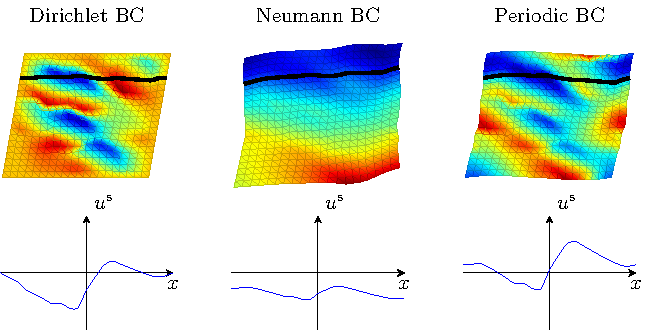
\includegraphics[width=0.75\textwidth]{img/subscaleBC.pdf}
    \caption{Different types of boundary conditions used on the RVE with the corresponding subscale fluctuation fields. From \cite{Sciegaj2020phd}.}
    \label{fig:bc_types}
\end{figure}

Those types differ in the way the macroscopic field is ``prolonged'' over the RVE, and the summary of differences can be found in \cite{Sciegaj2020phd}.
The bottom line is, given the macroscopic field that are to be prescribed on the RVE and the type of boundary condition, a complete RVE boundary value problem can be solved. 
The details of the implementation are outside the scope of this document, thus the focus is put on how to use the boundary conditions in OOFEM input files.

For the 3D RVE, \textbf{only} (strongly) periodic boundary conditions were considered in the project.
Those require a periodic mesh, and the use of boundary elements, as described in \cref{sec:3d}. 
No explicit boundary condition was implemented, as the macroscopic quantities are prescribed directly in the master node with conventional boundary conditions available in OOFEM.

In plane stress, \textbf{only} Dirichlet and Neumann type boundary conditions were implemented. 
Those can be used either in full FE$^2$ analyses (treated in \cref{sec:fe2}), or separately for convenient setup and solution of RVE problems. 
The implemented boundary conditions are:
\begin{itemize}
    \item \param{PrescribedDispSlipBCDirichletRC}, allowing for prescribing the macroscopic strain (optionally also macroscopic slip and slip gradient) on a reinforced concrete RVE using Dirichlet type boundary conditions
    \item \param{PrescribedDispSlipBCNeumannRC}, allowing for prescribing the macroscopic strain (optionally also macroscopic slip and slip gradient) on a reinforced concrete RVE using Neumann type boundary conditions
\end{itemize}

\subsection{PrescribedDispSlipBCDirichletRC}

The general syntax of \param{PrescribedDispSlipBCDirichletRC} boundary condition is the following:
\newline 

\begin{record}[0.85\textwidth]
    \recentry{\entKeywordInst{PrescribedDispSlipBCDirichletRC}}{\componentNum}
    \recentry{}{\field{loadTimeFunction}{in}}
    \recentry{}{\field{dofs}{ia}}
    \recentry{}{\optField{ccoord}{ra}}
    \recentry{}{\field{dispGrad}{rm}}
    \recentry{}{\optField{slip}{ra}}
    \recentry{}{\optField{slipGrad}{rm}}
    \recentry{}{\field{set}{in}}
    \recentry{}{\field{conboundset}{in}}
    \recentry{}{\optField{reinfxbound}{in}}
    \recentry{}{\optField{reinfybound}{in}}
\end{record}\\

\noindent The \param{PrescribedDispSlipBCDirichletRC} keyword is followed by the integer number (number of the BC). Next, the \param{loadTimeFunction} corresponding to the BC is specified, usually a \param{ConstantFunction}. 
Subsequently, the degrees of freedom integer array is specified after the keyword \param{dofs}. As the RVE problem is a plane stress problem, we consider the translations (dofs 1 and 2) and, if the reinforcement is modelled with beam elements, an optional rotation in the xy plane (dof 6).
The optional \param{ccoord} field specifies the coordinates of the centre of the RVE, and if not specified, it is set to the origin $(0,0)$.

The macroscopic fields are specified by keywords \param{dispGrad}, \param{slip}, and \param{slipGradient}, as described in \cref{sec:homogenization}. Note that the \param{dispGrad} field is required, but the \param{slip} and \param{slipGrad} fields are optional. This makes it possible to use the same boundary condition for different types of macroscopic problems - with and without the macroscopic reinforcement slip field.

The \param{conboundset} is the \param{elementboundaries} set which makes up the boundary of the RVE (light red in \cref{fig:dirichletsets}). This is used internally to compute the volume of the RVE when performing homogenization.
The last two sets - \param{reinfxbound} and \param{reinfybound} (green and lightblue in \cref{fig:dirichletsets}, respectively) - are required only if \param{slip} or \param{slipGradient} fields are present. These sets contain the boundary \textbf{nodes} of the reinforcement elements in $x$- and $y$-directions, respectively.
Currently, only orthogonal reinforcement layout aligned with $x$ and $y$ axes is supported.
The different types of the set are summarized in \cref{fig:dirichletsets}.

\begin{figure}[H]
    \centering
    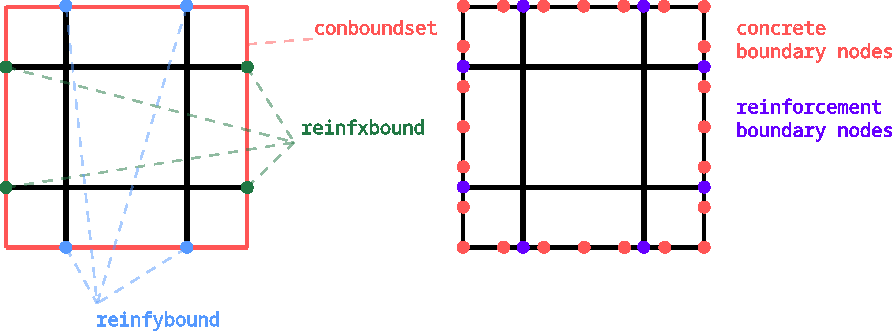
\includegraphics[width=0.8\textwidth]{img/dirichletsets.pdf}
    \caption{Summary of sets used in \param{PrescribedDispSlipBCDirichletRC}.}
    \label{fig:dirichletsets}
\end{figure}

The \param{set} field specifies the set onto which the Dirichlet boundary condition is to be applied. 
This can be either a set of boundary \param{nodes}, or \param{elementboundaries}, depending on intended use. 
It is noteworthy, that this BC can be applied either on the concrete solid, reinforcement bars or on both at the same time.
If the Dirichlet BC is only supposed to be prescribed only the concrete solid (not reinforcement), the set specified after the \param{set} keyword can be the same as the \param{conboundset}, which is a set of \param{elementboundaries} (light red in \cref{fig:dirichletsets}). Alternatively, a set of all concrete \param{nodes} on the boundary of the RVE can be used (corresponds to concrete boundary nodes in \cref{fig:dirichletsets}). This corresponds to Dirichlet-Neumann case described in \cref{sec:bc_applications}.

It is also possible to apply this BC only on the reinforcement bars.
In this case, the set of reinforcement boundary nodes (purple in \cref{fig:dirichletsets}) should be specified after the \param{set} keyword. 
This would correspond to Neumann-Dirichlet case from \cref{sec:bc_applications}, provided that an appropriate Neumann BC is used on the concrete boundary

Lastly, this BC can be applied on both concrete and reinforcement at the same time, corresponding to the Dirichlet-Dirichlet case from \cref{sec:bc_applications}. 
To do this, the set specified after the \param{set} keyword should contain all the nodes at concrete and reinforcement boundary, i.e., this set should be a union of concrete boundary nodes and reinforcement boundary nodes from \cref{fig:dirichletsets}.

\subsection{PrescribedDispSlipBCNeumannRC}

The general syntax of \param{PrescribedDispSlipBCNeumannRC} boundary condition is the following:
\newline

\begin{record}[0.85\textwidth]
    \recentry{\entKeywordInst{PrescribedDispSlipBCNeumannRC}}{\componentNum}
    \recentry{}{\field{loadTimeFunction}{in}}
    \recentry{}{\field{dofs}{ia}}
    \recentry{}{\optField{ccoord}{ra}}
    \recentry{}{\field{dispGrad}{rm}}
    \recentry{}{\optField{slip}{ra}}
    \recentry{}{\optField{slipGrad}{rm}}
    \recentry{}{\field{set}{in}}
    \recentry{}{\optField{concretevolset}{in}}
    \recentry{}{\optField{rebarsets}{ia}}
\end{record}\\

\noindent The \param{PrescribedDispSlipBCNeumannRC} keyword is followed by the integer number (number of the BC). Next, the \param{loadTimeFunction} corresponding to the BC is specified, usually a \param{ConstantFunction}. 
Subsequently, the degrees of freedom integer array is specified after the keyword \param{dofs}. As the RVE problem is a plane stress problem, we consider only the translations (dofs 1 and 2). 
This is due to the fact, that this BC prescribes the macroscopic strain only on the concrete volume, and not on the reinforcement. However, the optional macroscopic slip and slip gradients can be prescribed on the reinforcement bars.
The optional \param{ccoord} field specifies the coordinates of the centre of the RVE, and if not specified, it is set to the origin $(0,0)$.

The macroscopic fields are specified by keywords \param{dispGrad}, \param{slip}, and \param{slipGradient}, as described in \cref{sec:homogenization}. Note that the \param{dispGrad} field is required, but the \param{slip} and \param{slipGrad} fields are optional. This makes it possible to use the same boundary condition for different types of macroscopic problems - with and without the macroscopic reinforcement slip field.

The \param{set} field specifies the \param{elementboundaries} set of concrete boundaries (blue in \cref{fig:neumannsets}).
The last two sets - \param{concretevolset} and \param{rebarsets} - are required only if \param{slip} or \param{slipGradient} fields are present. 
The \param{concretevolset} set contains the all concrete \textbf{elements} in the volume of the RVE (light red in \cref{fig:neumannsets}).
The \param{rebarsets} field contains an integer array of reinforcement element sets, i.e., one set for all reinforcement bars going in the same direction (black in \cref{fig:neumannsets}).
For the RVE presented in \cref{fig:neumannsets}, all elements of the reinforcement bars in $x$-direction should be grouped in one set (light orange in \cref{fig:neumannsets}). Similarly, all elements of the reinforcement bars in $y$-direction should be grouped in another set (light violet in \cref{fig:neumannsets}). 
Those sets should then be given in the \param{rebarsets} field.
Currently, only orthogonal reinforcement layout aligned with $x$ and $y$ axes is supported.

The different types of the set are summarized in \cref{fig:neumannsets}.

\begin{figure}[H]
    \centering
    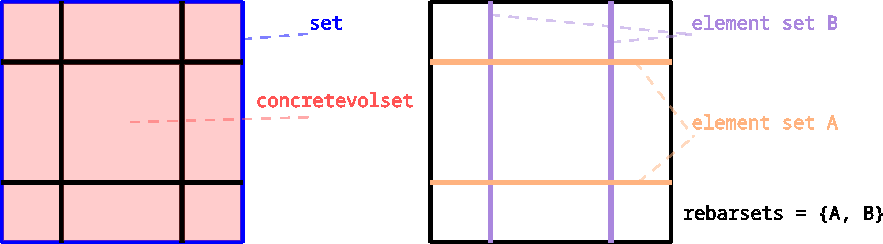
\includegraphics[width=0.8\textwidth]{img/neumannsets.pdf}
    \caption{Summary of sets used in \param{PrescribedDispSlipBCNeumannRC}.}
    \label{fig:neumannsets}
\end{figure}

\subsubsection{Pertinent test cases}
Following test cases can be studied for more insight: 
\begin{itemize}
    \item \texttt{rveDisp/2D/prescribeddispbcneumann01} - presribing a displacement gradient on a minimal solid RVE (\texttt{planestress2d} elements)
    \item \texttt{rveDisp/2D/prescribeddispbcneumann02} - presribing a displacement gradient on a minimal solid RVE (\texttt{trplanestress2d} elements)
    \item \texttt{rveDisp/2D/prescribeddispbcneumann03} - presribing a displacement gradient on a minimal solid RVE (\texttt{qplanestress2d} elements)
    \item \texttt{rveDisp/2D/prescribeddispbcneumann04} - presribing a displacement gradient on a minimal solid RVE (\texttt{qtrplstr} elements)
\end{itemize}

\subsection{TransverseReinforcementConstraint}
\label{sec:trc}

The transverse constraint between the concrete and reinforcement (specifying that there is no slip in the transverse direction between the materials) can be satisfied either strongly or weakly. 
Strong constraint involved tying concrete and steel nodes and requiring that the displacements in the transverse direction is equal for both.
This approach has been used in the project, as it was intuitive and did not require any additional implementation.

Another option is to satisfy the constraint \textit{weakly}. To do that, a Lagrange multiplier, which corresponds to a distributed load, is introduced on the bar. 
To use that constraint, a boundary condition class \texttt{TransverseReinforcementConstraint} has been implemented with the following use syntax:
\newline

\begin{record}[0.85\textwidth]
    \recentry{\entKeywordInst{TransverseReinforcementConstraint}}{\componentNum}
    \recentry{}{\field{loadTimeFunction}{in}}
    \recentry{}{\field{steelElSet}{in}}
    \recentry{}{\field{conElBoundSet}{in}}
\end{record}\\

The \texttt{TransverseReinforcementConstraint} boundary condition should be specified once for every single reinforcement bar.
\noindent The \param{TransverseReinforcementConstraint} keyword is followed by the integer number (number of the BC). Next, the \param{loadTimeFunction} corresponding to the BC is specified, usually a \param{ConstantFunction}.
\param{steelElSet} is a set of finite elements in the given reinforcement bar. 
\param{conElBoundSet} is a \param{elementboundaries} set of the boundaries of the plane stress concrete elements which are along the reinforcement bar, see \cref{fig:trcsets}. 
In the figure, a distance between the concrete and reinforcement has been added for clarity. Note that in the model, those nodes can be either coincident or very close to each other.

\begin{figure}[H]
    \centering
    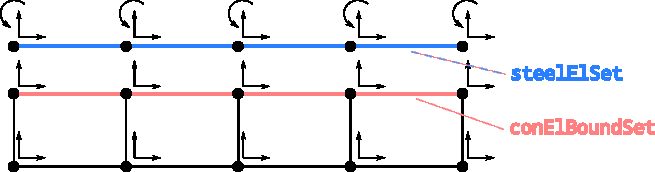
\includegraphics[width=0.75\textwidth]{img/trcsets.pdf}
    \caption{Summary of sets used in \param{TransverseReinforcementConstraint}.}
    \label{fig:trcsets}
\end{figure}


\noindent The following excerpt from the \texttt{transversereinfconstraint} test illustrates the use of this boundary condition:

\begin{minipage}{\linewidth}
\begin{lstlisting}[style=oofem,language=oofeminput]
# Elements of single reinforcement bar (vertical)
Set 9 elementranges { (101 110) }
# Elements of single reinforcement bar (horizontal)
Set 10 elementranges { (111 120) }
#Concrete element boundary set along horizontal bar
Set 14 elementboundaries 20 55 3 60 3 65 3 70 3 75 3 80 3 85 3 90 3 95 3 100 3
#Concrete element boundary set along vertical bar
Set 15 elementboundaries 20 76 4 77 4 78 4 79 4 80 4 5 3 10 3 15 3 20 3 25 3
# transverse constraints - one per reinforcement bar
TransverseReinforcementConstraint 2 loadTimeFunction 1 steelElSet 10 
                                    conElBoundSet 14
TransverseReinforcementConstraint 3 loadTimeFunction 1 steelElSet 9 
                                    conElBoundSet 15
\end{lstlisting}
\end{minipage}

\subsubsection{Pertinent test cases}
The following test case can be studied for more insight:
\begin{itemize}
    \item \texttt{rveDispSlip/2D/transversereinfconstraint} - weak transverse reinforcement constraint on a reinforced concrete RVE
\end{itemize}

\subsection{Application examples}
\label{sec:bc_applications}

\subsubsection{Macroscopic strain}

As described in \cite{PaperA}, different types of boundary conditions can be chosen to be applied on the concrete and reinforcement parts of the RVE. 
This gives four different possibilities, as shown in \cref{fig:bc_combs}.

\begin{figure}[H]
    \centering
    \def\svgwidth{0.75\textwidth}
    \import{img}{bcs.pdf_tex}
    \caption{Combinations of boundary conditions used in a reinforced concrete RVE. From \cite{PaperA}.}
    \label{fig:bc_combs}
\end{figure}

\noindent To summarize, the use of the pertinent boundary conditions has been demonstrated in \cref{lst:rveDisp}, which contains excerpts from test cases \texttt{rveDisp01}-\texttt{rveDisp04}. Note that the set numbers vary between the examples, and the input files should be studied for more insight.

\begin{minipage}{\linewidth}
\begin{lstlisting}[style=oofem,language=oofeminput, caption={Use of boundary condition for prescribing a macroscopic strain tensor.}, label=lst:rveDisp]
# Dirichlet-Dirichlet
PrescribedDispSlipBCDirichletRC 1 loadTimeFunction 1 dofs 3 1 2 6 
    ccoord 3 0.0 0.0 0.0 dispGrad 2 2 {0.3e-9 0.4e-9; 0.4e-9 -0.5e-9} 
    set 5 conboundset 6

# Dirichlet-Neumann
PrescribedDispSlipBCDirichletRC 1 loadTimeFunction 1 dofs 3 1 2 6 
    ccoord 3 0.0 0.0 0.0 dispGrad 2 2 {0.3e-9 0.4e-9; 0.4e-9 -0.5e-9} 
    set 6 conboundset 6

# Neumann-Dirichlet
PrescribedDispSlipBCNeumannRC 1 loadTimeFunction 1 dofs 2 1 2 
    ccoord 3 0.0 0.0 0.0 dispGrad 2 2 {0.3e-9 0.4e-9; 0.4e-9 -0.5e-9} 
    set 5
PrescribedDispSlipBCDirichletRC 2 loadTimeFunction 1 dofs 3 1 2 6 
    ccoord 3 0.0 0.0 0.0 dispGrad 2 2 {0.3e-9 0.4e-9; 0.4e-9 -0.5e-9} 
    set 6 conboundset 5

# Neumann-Neumann
PrescribedDispSlipBCNeumannRC 1 loadTimeFunction 1 dofs 2 1 2 
    ccoord 3 0.0 0.0 0.0 dispGrad 2 2 {0.3e-9 0.4e-9; 0.4e-9 -0.5e-9} set 5

\end{lstlisting}
\end{minipage}
The pertinent test cases are presented in the \cref{tab:rveDisp} below. 
The columns specify which type of boundary condition was used on the concrete and reinforcement part of the RVE.

\begin{table}[H]
    \caption{Test cases on a reinforced concrete RVE, prescribing a macroscopic strain tensor.}
    \centering
\begin{tabular}{|l|l|l|}
\hline
 Test case   & Concrete BC  & Reinforcement BC \\ \hline
\texttt{rveDisp/2D/rveDisp01} & Dirichlet & Dirichlet     \\ \hline
\texttt{rveDisp/2D/rveDisp02} & Dirichlet & Neumann       \\ \hline
\texttt{rveDisp/2D/rveDisp03} & Neumann   & Dirichlet     \\ \hline
\texttt{rveDisp/2D/rveDisp04} & Neumann   & Neumann       \\ \hline
\end{tabular}
\label{tab:rveDisp}
\end{table}


\subsubsection{Macroscopic strain, slip and slip gradient}

As previously alluded to, the implemented boundary conditions can also prescribe macroscopic slip and slip gradient. 
Similar as before, each macroscopic quantity can be prescribed either with Dirichlet, Neumann boundary condition, or not prescribed at all. 
To summarize, the use of the pertinent boundary conditions has been demonstrated in \cref{lst:rveDispSlip}, which contains excerpts from test cases \texttt{rveDispSlip07}-\texttt{rveDispSlip10}. Note that the set numbers vary between the examples, and the input files should be studied for more insight.

\begin{minipage}{\linewidth}
\begin{lstlisting}[style=oofem,language=oofeminput, caption={Use of boundary condition for prescribing macroscopic strain, slip and slip gradient.}, label=lst:rveDispSlip]
# Dirichlet-Dirichlet-Dirichlet
PrescribedDispSlipBCDirichletRC 1 loadTimeFunction 1 dofs 3 1 2 6 
    ccoord 3 0.0 0.0 0.0 dispGrad 2 2 {0.3e-6 0.4e-6; 0.4e-6 -0.5e-6} 
    slip 2 1e-5 -2e-5 slipGrad 2 2 {0.3e-6 0.4e-6; 0.4e-6 -0.5e-6} 
    set 5 conboundset 6 reinfxbound 8 reinfybound 7

# Neumann-Neumann-Neumann
PrescribedDispSlipBCNeumannRC 1 loadTimeFunction 1 dofs 2 1 2 
    ccoord 3 0.0 0.0 0.0 dispGrad 2 2 {0.3e-6 0.4e-6; 0.4e-6 -0.5e-6} 
    slip 2 1e-5 -2e-5 slipGrad 2 2 {0.3e-6 0.4e-6; 0.4e-6 -0.5e-6} 
    set 6 concretevolset 1 rebarsets 2 9 10

# Dirichlet-Neumann-Neumann
PrescribedDispSlipBCDirichletRC 1 loadTimeFunction 1 dofs 2 1 2 
    ccoord 3 0.0 0.0 0.0 dispGrad 2 2 {0.3e-6 0.4e-6; 0.4e-6 -0.5e-6} 
    set 6 conboundset 6
PrescribedDispSlipBCNeumannRC 2 loadTimeFunction 1 dofs 2 1 2 
    ccoord 3 0.0 0.0 0.0 slip 2 1e-5 -2e-5 
    slipGrad 2 2 {0.3e-6 0.4e-6; 0.4e-6 -0.5e-6} set 6 concretevolset 1 
    rebarsets 2 9 10

# Neumann-Dirichlet-Dirichlet
PrescribedDispSlipBCNeumannRC 1 loadTimeFunction 1 dofs 2 1 2 
    ccoord 3 0.0 0.0 0.0 dispGrad 2 2 {0.3e-6 0.4e-6; 0.4e-6 -0.5e-6} set 6 
PrescribedDispSlipBCDirichletRC 2 loadTimeFunction 1 dofs 3 1 2 6 
    ccoord 3 0.0 0.0 0.0 slip 2 1e-5 -2e-5 
    slipGrad 2 2 {0.3e-6 0.4e-6; 0.4e-6 -0.5e-6} 
    set 15 conboundset 6 reinfxbound 8 reinfybound 7

\end{lstlisting}
\end{minipage}
The pertinent test cases are presented in the \cref{tab:rveDispSlip} below. 
The columns specify which type of boundary condition was used to prescribe a specific macroscopic component.

\begin{table}[H]
    \centering
    \caption{Test cases on a reinforced concrete RVE, prescribing macroscopic strain, slip and slip gradient.}
\begin{tabular}{|l|l|l|l|}
\hline
   Test case      & $\bm{\bar{\varepsilon}}$ & $\bm{\bar{s}}$ & $\bm{\bar{g}}$ \\ \hline
\texttt{rveDispSlip/2D/rveDispSlip01} & -                   & Dirichlet & -         \\ \hline
\texttt{rveDispSlip/2D/rveDispSlip02} & -                   & -         & Dirichlet \\ \hline
\texttt{rveDispSlip/2D/rveDispSlip03} & -                   & Neumann   & -         \\ \hline
\texttt{rveDispSlip/2D/rveDispSlip04} & -                   & -         & Neumann   \\ \hline
\texttt{rveDispSlip/2D/rveDispSlip05} & -                   & Dirichlet & Dirichlet \\ \hline
\texttt{rveDispSlip/2D/rveDispSlip06} & -                   & Neumann   & Neumann   \\ \hline
\texttt{rveDispSlip/2D/rveDispSlip07} & Dirichlet           & Dirichlet & Dirichlet \\ \hline
\texttt{rveDispSlip/2D/rveDispSlip08} & Neumann             & Neumann   & Neumann   \\ \hline
\texttt{rveDispSlip/2D/rveDispSlip09} & Dirichlet           & Neumann   & Neumann   \\ \hline
\texttt{rveDispSlip/2D/rveDispSlip10} & Neumann             & Dirichlet & Dirichlet \\ \hline
\end{tabular}
\label{tab:rveDispSlip}
\end{table}



\clearpage
\section{FE$^2$ analysis}
\label{sec:fe2}

In an FE$^2$ analysis, an RVE problem is solved for each integration point in the macroscopic model, see \cref{fig:fe2}. The macroscopic fields are prescribed on the RVE via suitable boundary conditions (see \cref{sec:bc}), and the effective work conjugates (e.g., stresses) are homogenized and brought back to the macroscale. The analysis then continues. 
As such, the multiscale method can be viewed as a complex material model, which for given input (e.g., strain tensor) provides the output (e.g., stress tensor). 
However, apart from the macroscopic response, we also have access to subscale results, and can study in detail the progression of damage in individual RVEs.

The RVE input file must fulfil certain requirements:
\begin{itemize}
    \item it must have a \texttt{PrescribedDispSlip*} boundary condition,
    \item the \texttt{PrescribedDispSlip*} must be the first boundary condition,
    \item the fields \param{dispGrad}, \param{slip}, and \param{slipGrad} must be specified. However, as the macroscopic components will be propagated directly from the macroscopic problem (and are not known in advance), the values for those input fields should be 0, e.g., 
    \begin{lstlisting}[style=oofem,language=oofeminput]
PrescribedDispSlipBCDirichletRC 1 loadTimeFunction 1 dofs 3 1 2 6 
    ccoord 3 0.0 0.0 0.0 dispGrad 2 2 {0 0; 0 0} slip 2 0 0 
    slipGrad 2 2 {0 0; 0 0} set 5 conboundset 6 reinfxbound 8 reinfybound 7
    \end{lstlisting}
\end{itemize}



\subsection{StructSlipFE2Material}

In OOFEM, the FE$^2$ analysis is possible with the \param{StructSlipFE2Material} material model assigned to macroscopic finite element. 
This material requires the RVE model, given in the form of OOFEM input file. 
Each \param{StructSlipFE2Material} material requires one RVE model, but several different RVEs can be used throughout the macroscopic model (as in \cite{Sciegaj2019semc}). In that case, different \param{StructSlipFE2Material} models should be assigned to different finite elements in the macroscopic problem. 
The syntax of the model is as follows:
\newline

\begin{record}[0.85\textwidth]
    \recentry{\entKeywordInst{StructSlipFE2Material}}{\componentNum}
    \recentry{}{\field{filename}{s}}
    \recentry{}{\optFieldFlag{export\_all\_gps}{}}
    \recentry{}{\optField{output\_selected\_el\_gps}{ia}}
    \recentry{}{\optFieldFlag{use\_num\_tangent}{}}
    \recentry{}{\optFieldFlag{use\_ext\_stiffness}{}}
    \recentry{}{\optField{dSdE}{rm}}
    \recentry{}{\optField{dBSdE}{rm}}
    \recentry{}{\optField{dRSdE}{rm}}
    \recentry{}{\optField{dSdS}{rm}}
    \recentry{}{\optField{dBSdS}{rm}}
    \recentry{}{\optField{dRSdS}{rm}}
    \recentry{}{\optField{dSdG}{rm}}
    \recentry{}{\optField{dBSdG}{rm}}
    \recentry{}{\optField{dRSdG}{rm}}
\end{record}\\

\noindent The \param{StructSlipFE2Material} keyword is followed by the integer number (number of the material). 
Next, and most important the name of the input file for the RVE model is specified after the \param{filename} keyword. The rest of the keywords is optional.  
The minimal syntax is illustrated below:

\begin{lstlisting}[style=oofem, language=oofeminput]
StructSlipFE2Material 1 d 1.0 filename fe2disprve1x1dd.in.rve 
\end{lstlisting}

\noindent In the above, the RVE model is stored in the file \texttt{fe2disprve1x1dd.in.rve}, located in the same directory as the macroscopic model. 
If output modules are specified in the RVE file (e.g., \texttt{vtkxml} or \texttt{matlab} output modules), only the results for one RVE (last one when iterating over model Gauss points) will be created by default (with the output file suffex with \texttt{\_el1\_gp1}).
This behaviour can be changed by using the \param{export\_all\_gps} flag:

\begin{lstlisting}[style=oofem, language=oofeminput]
StructSlipFE2Material 1 d 1.0 filename fe2disprve1x1dd.in.rve export_all_gps
\end{lstlisting}

\noindent This way, the results from all Gauss points will be stored in separate files.
Note that this will produce a large amount of files, make sure that there is enough space for them.
An alternative is to output results only from selected Gauss points.
This can be done by specyfing the integer array of finite element and Gauss point numbers after the keyword \param{output\_selected\_el\_gps}, e.g., the following syntax

\begin{lstlisting}[style=oofem, language=oofeminput]
StructSlipFE2Material 1 d 1.0 filename fe2disprve1x1dd.in.rve 
                        output_selected_el_gps 6 20 3 21 1 23 4
\end{lstlisting}
will output the results from Gauss point 3 in element 20, Gauss point 1 in element 21, and Gauss point 4 in element 23.

When solving nonlinear problems, Newton-Raphson iterations are usually used in OOFEM. Computing of tangent stiffness matrix is then handled by the material model directly. In case of the RVE problem, this should be implemented by the corresponding boundary conditions. By default, the material will use the tangent implemented by the boundary condition. 
However, as this is usually a complex task, the extact computation of the tangent is often omitted. 
In this case, we can either compute the tangent numerically, or supply a value directly (useful for e.g., modified Newton iterations with linear stiffness).
To compute the tangent numerically, the \param{use\_num\_tangent} should be specified:

\begin{lstlisting}[style=oofem, language=oofeminput]
StructSlipFE2Material 1 d 1.0 filename fe2disprve1x1dd.in.rve use_num_tangent
\end{lstlisting}
Note that this will result in the model computing the tangent stiffness via numerical perturbation (i.e., solving a new RVE problem for each component of the tangent). This means solving many RVE problems for each Gauss point in each element. 
The overall computation time is therefore increased substantially.

Another option is for the user to provide the tangent stiffness directly (e.g., by performing the numerical perturbation on a single RVE off-line before the analysis). To do this, the \param{use\_ext\_stiffness} flag should be used, followed by the tangent stiffness matrices pertinent to the problem.
After the keyword, the tangents pertinent to the macroscopic problem should be specified as matrices.
Note that the plane stress problem requires only one tangent, whereas the addition of macroscopic reinforcement slip field increases the number of required tangents to 9.
The required tangent keywords, their mathematical expression and their dimensions are summarized in \cref{tab:tangents}. In plane stress, only the \param{dsde} tangent is necessary, see \cref{lst:tangent_disp} and \ref{lst:tangent_slip}.

\begin{table}[H]
    \renewcommand*{\arraystretch}{3}
    \caption{Tangent stifness matrices that can be supplied to \param{StructSlipFE2Material} material.}
    \centering
    \begin{tabular}{|l|c|c|l|c|c|l|c|c|}
        \hline
    keyword & symbol & dim &  keyword  & symbol & dim &  keyword & symbol & dim \\ \hline
    \param{dSdE}  & $\dfrac{\bm{\bar{\sigma}}}{\bm{\bar{\varepsilon}}}$ & $3\times3$  & \param{dSdS} & $\dfrac{\bm{\bar{\sigma}}}{\bm{\bar{s}}}$ & $3\times2$  & \param{dSdG} & $\dfrac{\bm{\bar{\sigma}}}{\bm{\bar{g}}}$ & $3\times4$  \\ \hline
    \param{dBSdE} & $\dfrac{\bm{\bar{\tau}_b}}{\bm{\bar{\varepsilon}}}$ & $2\times3$  & \param{dBSdS} & $\dfrac{\bm{\bar{\tau}_b}}{\bm{\bar{s}}}$ & $2\times2$  & \param{dBSdG} & $\dfrac{\bm{\bar{\tau}_b}}{\bm{\bar{g}}}$ & $2\times4$  \\ \hline
    \param{dRSdE} & $\dfrac{\bm{\bar{\sigma}_s}}{\bm{\bar{\varepsilon}}}$ & $4\times3$  & \param{dRSdS} & $\dfrac{\bm{\bar{\sigma}_s}}{\bm{\bar{s}}}$ & $4\times2$  & \param{dRSdG} &  $\dfrac{\bm{\bar{\sigma}_s}}{\bm{\bar{g}}}$ & $4\times4$ \\ \hline
    \end{tabular}
    \label{tab:tangents}
\end{table}


\begin{lstlisting}[style=oofem,language=oofeminput, caption={Syntax for providing tangent stiffness for macroscopic plane stress problem}, label=lst:tangent_disp]
# macroscopic plane stress problem
StructSlipFE2Material 1 d 1.0 filename fe2disprve1x1dd.in.rve use_ext_stiffness 
                        dSdE 3 3 {36.2507e+09	6.9323e+09	2.9505e+02; 
                                  6.9323e+09	34.9136e+09	-2.3936e+03; 
                                  2.9505e+02	-2.3936e+03	13.8658e+09}
\end{lstlisting}

\begin{minipage}{0.9\textwidth}
\begin{lstlisting}[style=oofem, language=oofeminput, caption={Syntax for providing tangent stiffness for macroscopic plane stress with effective reinforcement slip field}, label=lst:tangent_slip]
# macroscopic plane stress with reinforcement slip field
StructSlipFE2Material 1 d 1.0 filename fe2dispsliprve1x1dd.in.rve use_ext_stiffness 
            dSdE 3 3 { 3.6250e+10  6.9323e+09  2.9505e+02; 
                    6.9323e+09  3.4913e+10  -2.3936e+03; 
                    2.9505e+02  -2.3936e+03  1.3865e+10} 
            dBSdE 2 3 { 7.5564e+05  1.4917e+05  -4.6064e+07; 
                    -2.7273e+05  -1.3649e+06  2.2506e+06 } 
            dRSdE 4 3 { 1.5706e+09  3.4606e+05  -9.6819e+02; 
                    -6.8920e+04  2.5083e+08  -3.1767e+02; 
                        0.0000e+00  0.0000e+00  0.0000e+00; 
                        0.0000e+00  0.0000e+00  0.0000e+00 } 
            dSdS 3 2 { 7.5564e+05  -2.7273e+05; 
                    1.4917e+05  -1.3649e+06; 
                    -4.6064e+07  2.2506e+06 } 
            dBSdS 2 2 {  7.9177e+10  4.7826e+03; 
                        4.7826e+03  2.6249e+10  } 
            dRSdS 4 2 { -5.4548e+03  1.2422e+05; 
                        -2.2920e+04  4.0332e+03; 
                        0.0000e+00  0.0000e+00; 
                        0.0000e+00  0.0000e+00 } 
            dSdG 3 4 {  1.5706e+09  -6.8920e+04  0.0000e+00  0.0000e+00; 
                        3.4606e+05  2.5083e+08  0.0000e+00  0.0000e+00; 
                    -9.6819e+02  -3.1767e+02  0.0000e+00  0.0000e+00  } 
            dBSdG 2 4 { -5.4548e+03  -2.2920e+04  0.0000e+00  0.0000e+00; 
                        1.2422e+05  4.0332e+03  0.0000e+00  0.0000e+00 } 
            dRSdG 4 4 { 1.8773e+09  9.6766e+04  0.0000e+00  0.0000e+00; 
                        9.6766e+04  3.6845e+08  0.0000e+00  0.0000e+00; 
                        0.0000e+00  0.0000e+00  0.0000e+00  0.0000e+00; 
                        0.0000e+00  0.0000e+00  0.0000e+00  0.0000e+00 }
\end{lstlisting}
\end{minipage}


\subsection{PrescribedDispSlipMultiple}

As already mentioned in the beginning of \cref{sec:fe2}, the \texttt{PrescribedDispSlip*} boundary condition should be specified as the first one in the RVE model. 
Implicitly, the displacement (and potentially slip) gradient will be passed to this boundary condition in the course of the multiscale analysis. 
However, if more than one boundary conditions need to be specified on parts of the RVE (e.g., in the Neummann-Dirichlet case), the second boundary condition will not be automatically used by the code. 
For this reason, a \texttt{PrescribedDispSlipMultiple} wrapper, allowing for use of multiple boundary conditions in the RVE problem, was implemented.
The syntax of the wrapper is the following:
\newline

\begin{record}[0.85\textwidth]
    \recentry{\entKeywordInst{PrescribedDispSlipMultiple}}{\componentNum}
    \recentry{}{\field{bcs}{ia}}
    \recentry{}{\field{loadTimeFunction}{in}}
\end{record}\\

\noindent The boundary conditions which are to be used for the RVE are specified in the integer array after the \texttt{bcs} keyword. 
The \texttt{PrescribedDispSlipMultiple} wrapper acts as the one required \texttt{PrescribedDispSlip*} boundary conditionin the RVE.
The pertinent gradients (and fields) are then autmatically passed to the boundary conditions specified by the wrapper.
For instance, 
a set of two boundary conditions (numbered 2 and 3) can be used in the FE$^2$ analysis using the following syntax: 

\begin{lstlisting}[style=oofem,language=oofeminput]
PrescribedDispSlipMultiple 1 bcs 2 2 3 loadTimeFunction 1
PrescribedDispSlipBCNeumannRC 2 loadTimeFunction 1 dofs 2 1 2 
    ccoord 3 0.0 0.0 0.0 dispGrad 2 2 {0 0; 0 0} set 5
PrescribedDispSlipBCDirichletRC 3 loadTimeFunction 1 dofs 3 1 2 6 
    ccoord 3 0.0 0.0 0.0 dispGrad 2 2 {0 0; 0 0} set 6 conboundset 5
\end{lstlisting}

The following test case can be studied for more insight:
\begin{itemize}
    \item \texttt{fe2Disp/planeStress/deepbeam03} - FE$^2$ analysis of a deep beam using Neumann-Dirichlet boundary conditions, from \cite{PaperA}.
\end{itemize}

\subsection{UserDefDirichletBC}

Sometimes, the full FE$^2$ analysis is just too much, as only results from a single RVE are necessary, e.g., to study crack growth. 
However, it's usually not possible to predict and describe the strain evolution with a single \texttt{loadTimeFunction}. Furthermore, the evolution of individual tensor components adds complexity to this task.
To overcome this limitation, a way of prescribing a given strain (or potentially also slip) history on a single RVE is needed. 
To do this, a mock FE$^2$ analysis can be used. In the mock analysis, only one macroscopic element can be defined. 

The challenge now is to prescribe deformation history on the macroscopic nodes, such that the strains ($\bm{\varepsilon}$) computed at the locations of the chosen Gauss point are equal to the given strain history. In case of macroscopic slip field, we also need to prescribe a slip history, so that the given slip ($\bm{s}$) and slip gradient ($\bm{g}$) will be propagated into the Gauss point. This can be done in many ways, and the parent macroscopic elements chosen in the project are shown in \cref{fig:fakefe2}.

\begin{figure}[H]
    \centering
    \def\svgwidth{0.8\textwidth}
    \import{img}{fakefe2disp.pdf_tex}
    \caption{Parent macroscopic elements for mock FE$^2$ analyses.}
    \label{fig:fakefe2}
\end{figure}

\noindent By prescribing specific displacement (and slip) values in specific nodes, the given strain (as well as slip and slip gradient) values will be propagated into the Gauss point (marked in blue). The choices made in the project are summarized in \cref{tab:fakefe2disp} for the \texttt{trplanestress2d} element, and in \cref{tab:fakefe2dispslip} for the \texttt{qtrplstrslip} element.

\begin{table}[H]
    \centering
    \caption{Prescribed displacement values in the nodes of \texttt{trplanestress2d} element.}
    \begin{tabular}{|c|c|c|}
    \hline
    \textbf{Node} & $u$                                      & $v$                    \\ \hline
    1    & $0$                                        & $0$                      \\ \hline
    2    & $\bar{\varepsilon}_{xx}$                   & $0$                      \\ \hline
    3    & $\bar{\varepsilon}_{xx}+\bar{\gamma}_{xy}$ & $\bar{\varepsilon}_{yy}$ \\ \hline
    \end{tabular}
    \label{tab:fakefe2disp}
\end{table}

\begin{table}[H]
    \centering
    \caption{Prescribed displacement and slip values in the nodes of \texttt{qtrplstrslip} element.}
    \begin{tabular}{|c|c|c|c|c|}
    \hline
    \textbf{Node} & $u$ & $v$ & $s_x$ & $s_y$ \\ \hline
    1    & $0$   & $0$    & $-2\bar{g}_{xx} - \bar{g}_{xy} - 3\bar{s}_x$      &  $-2\bar{g}_{yx} - \bar{g}_{yy} - 3\bar{s}_y$      \\ \hline
    2    & $3\bar{\varepsilon}_{xx}$    & $3\bar{\gamma}_{xy} + 3\bar{\varepsilon}_{xx}$    &  $\bar{g}_{xx} - \bar{g}_{xy} - 3\bar{s}_x$     & $\bar{g}_{yx} - \bar{g}_{yy} - 3\bar{s}_y$      \\ \hline
    3    & $0$    & $3\bar{\gamma}_{xy} + 3\bar{\varepsilon}_{xx} +3\bar{\varepsilon}_{yy}$    & $\bar{g}_{xx} + 2\bar{g}_{xy} - 3\bar{s}_x$      & $\bar{g}_{yx} + 2\bar{g}_{yy} - 3\bar{s}_y$      \\ \hline
    4    & $0$    & $0$    &  $0$     &  $0$     \\ \hline
    5    & $0$    & $0$    &  $0$     &  $0$     \\ \hline
    6    & $0$    & $0$    &  $0$     &  $0$     \\ \hline
    \end{tabular}
    \label{tab:fakefe2dispslip}
\end{table}

\noindent Prescribing the displacement and slip values given above ensures that the strain, slip and slip gradients in the marked Gauss point are:

\begin{align*}
    \bm{\bar{\varepsilon}} &= \left[ \bar{\varepsilon}_{xx}, \quad \bar{\varepsilon}_{yy}, \quad \bar{\gamma}_{xy} \right] \\
    \bm{\bar{s}} &= \left[ \bar{s}_x, \quad \bar{s}_y \right]\\
    \bm{\bar{g}} &= \left[ \bar{g}_{xx}, \quad \bar{g}_{yy}, \quad \bar{g}_{xy}, \quad \bar{g}_{yx} \right]
\end{align*}
To prescribe a specific time-history value in a node, the \texttt{UserDefDirichletBC} boundary condition can be used. 
This boundary condition allows the user to write a Python function named \texttt{giveUserDefBC}, which returns the value for a given node at a given time and for a specific degree of freedom. 
The use syntax of \texttt{UserDefDirichletBC} is:
\newline

\begin{record}[0.85\textwidth]
    \recentry{\entKeywordInst{UserDefDirichletBC}}{\componentNum}
    \recentry{}{\field{loadTimeFunction}{in}}
    \recentry{}{\field{filename}{s}}
\end{record}\\

\noindent The most important input field is the \texttt{filename}, which specifies the Python file with the function \texttt{giveUserDefBC}. 
In the following example, three different \param{UserDefDirichletBC} boundary conditions are used in three different nodes. 
The corresponding functions are located in the files \texttt{bcnode1.py}, \texttt{bcnode2.py}, and \texttt{bcnode3.py}. 

\begin{lstlisting}[style=oofem, language=oofeminput]
# node definition
node 1 coords 3 0 0 0 dofidmask 4 1 2 51 52 bc 4 1 1 1 1
node 2 coords 3 1 0 0 dofidmask 4 1 2 51 52 bc 4 2 2 2 2
node 3 coords 3 1 1 0 dofidmask 4 1 2 51 52 bc 4 3 3 3 3 

# bc definition
UserDefDirichletBC 1 loadTimeFunction 1 filename bcnode1
UserDefDirichletBC 2 loadTimeFunction 1 filename bcnode2
UserDefDirichletBC 3 loadTimeFunction 1 filename bcnode3
\end{lstlisting}

\noindent The \texttt{giveUserDefBC} function takes the node coordinates, the degree of freedom and the time step as arguments and returns a single value which is to be prescribed in the node. The function prototype is given below:
\begin{lstlisting}[style=mystyle, language=Python]
def giveUserDefBC(iCoords, iDofNum, iTime):
    prescribedValue = ...
    return prescribedValue
\end{lstlisting}
 For example implementations, the pertinent Python files of the test cases \texttt{fakefe2*} can be consulted. The implemented function reads input from a text file. This is of course, only one possible solution, the freedom is left to the user. It is noteworthy, that for the \texttt{UserDefDirichletBC} boundary condition to work, OOFEM must be compiled with Python support, i.e., the flag \texttt{USE\_PYTHON\_EXTENSION} must be on during CMake configuration. Following test cases can be studied for more insight:
\begin{itemize}
    \item \texttt{fe2Disp/planeStress/fakefe2disp} - prescribed strain history on an RVE with Dirichlet-Dirichlet boundary conditions. Presented in \cite{PaperA} and \cite{PaperB}.
    \item \texttt{fe2DispSlip/planeStress/fakefe2dispslip01} - prescribed strain, slip and slip gradient history on an RVE with Dirichlet-Dirichlet-Dirichlet boundary conditions. Presented in \cite{PaperB} and \cite{PaperC}.
    \item \texttt{fe2DispSlip/planeStress/fakefe2dispslip02} - prescribed strain, slip and slip gradient history on an RVE with Dirichlet-Neumann-Neumann boundary conditions. Presented in \cite{PaperC}.
\end{itemize}
\subsection{Application examples}
\label{sec:fe2_applications}

\subsubsection{Macroscopic strain}

Following test cases can be studied for more insight:
\begin{itemize}
    \item \texttt{fe2Disp/planeStress/deepbeam01} - FE$^2$ analysis of a reinforced concrete deep beam with Dirichlet-Dirichlet subscale boundary conditions. Presented in \cite{PaperA}.
    \item \texttt{fe2Disp/planeStress/deepbeam02} - FE$^2$ analysis of a reinforced concrete deep beam with Dirichlet-Neumann subscale boundary conditions. Presented in \cite{PaperA}.
    \item \texttt{fe2Disp/planeStress/deepbeam03} - FE$^2$ analysis of a reinforced concrete deep beam with Neumann-Dirichlet subscale boundary conditions. Presented in \cite{PaperA}.
    \item \texttt{fe2Disp/planeStress/deepbeam04} - FE$^2$ analysis of a reinforced concrete deep beam with Neumann-Neumann subscale boundary conditions. Presented in \cite{PaperA}.
    \item \texttt{fe2Disp/planeStress/aci-i} - FE$^2$ analysis of the ACI-I beam with Dirichlet-Dirichlet subscale boundary conditions and multiple RVEs over the macroscopic domains. Presented in \cite{Sciegaj2019semc}.
    \item \texttt{fe2Disp/planeStress/stm-m} - FE$^2$ analysis of the STM-M beam with Dirichlet-Dirichlet subscale boundary conditions and multiple RVEs over the macroscopic domains. Presented in \cite{Sciegaj2019semc}.
    \item \texttt{fe2Disp/planeStress/wt-4} - FE$^2$ analysis of the WT4 beam with Dirichlet-Dirichlet subscale boundary conditions and multiple RVEs over the macroscopic domains. Presented in \cite{Sciegaj2019semc}.
\end{itemize}

\subsubsection{Macroscopic strain, slip and slip gradient}

Following test cases can be studied for more insight:
\begin{itemize}
    \item \texttt{fe2DispSlip/planeStress/deepbeam01} - FE$^2$ analysis of a reinforced concrete deep beam with Dirichlet-Dirichlet-Dirichlet subscale boundary conditions. Presented in \cite{PaperB}.
    \item \texttt{fe2Disp/planeStress/deepbeam02} - FE$^2$ analysis of a reinforced concrete deep beam with Dirichlet-Neumann-Neumann subscale boundary conditions. Presented in \cite{PaperC}.
\end{itemize}

\clearpage

\addcontentsline{toc}{section}{References}
\printbibliography

\end{document}
